\documentclass[a4paper]{article}
\usepackage[margin=3.5cm]{geometry}
\usepackage{amsmath}
\usepackage{amssymb}
\usepackage[svgnames]{xcolor}
\usepackage{amsthm}
\usepackage{dsfont}
\usepackage{graphicx}
\usepackage{hyperref}
\usepackage{datetime}
\usepackage{outlines}
\usepackage{float}
\usepackage{booktabs}
\usepackage{enumitem}


\definecolor{fgcolor}{rgb}{0.345, 0.345, 0.345}
\newcommand{\hlnum}[1]{\textcolor[rgb]{0.686,0.059,0.569}{#1}}%
\newcommand{\hlstr}[1]{\textcolor[rgb]{0.192,0.494,0.8}{#1}}%
\newcommand{\hlcom}[1]{\textcolor[rgb]{0.678,0.584,0.686}{\textit{#1}}}%
\newcommand{\hlopt}[1]{\textcolor[rgb]{0,0,0}{#1}}%
\newcommand{\hlstd}[1]{\textcolor[rgb]{0.345,0.345,0.345}{#1}}%
\newcommand{\hlkwa}[1]{\textcolor[rgb]{0.161,0.373,0.58}{\textbf{#1}}}%
\newcommand{\hlkwb}[1]{\textcolor[rgb]{0.69,0.353,0.396}{#1}}%
\newcommand{\hlkwc}[1]{\textcolor[rgb]{0.333,0.667,0.333}{#1}}%
\newcommand{\hlkwd}[1]{\textcolor[rgb]{0.737,0.353,0.396}{\textbf{#1}}}%
\let\hlipl\hlkwb

\usepackage{framed}
\makeatletter
\newenvironment{kframe}{%
 \def\at@end@of@kframe{}%
 \ifinner\ifhmode%
  \def\at@end@of@kframe{\end{minipage}}%
  \begin{minipage}{\columnwidth}%
 \fi\fi%
 \def\FrameCommand##1{\hskip\@totalleftmargin \hskip-\fboxsep
 \colorbox{shadecolor}{##1}\hskip-\fboxsep
     % There is no \\@totalrightmargin, so:
     \hskip-\linewidth \hskip-\@totalleftmargin \hskip\columnwidth}%
 \MakeFramed {\advance\hsize-\width
   \@totalleftmargin\z@ \linewidth\hsize
   \@setminipage}}%
 {\par\unskip\endMakeFramed%
 \at@end@of@kframe}
\makeatother

\definecolor{shadecolor}{rgb}{.97, .97, .97}
\definecolor{messagecolor}{rgb}{0, 0, 0}
\definecolor{warningcolor}{rgb}{1, 0, 1}
\definecolor{errorcolor}{rgb}{1, 0, 0}
\newenvironment{knitrout}{}{} % an empty environment to be redefined in TeX


% code highlighting
\usepackage{minted}
\usepackage{xpatch}
\newminted[cminted]{python}{fontsize=\small}
\xpretocmd{\cminted}{\RecustomVerbatimEnvironment{Verbatim}{BVerbatim}{}}{}{}

% link coloring
%\hypersetup{
%    colorlinks,
%    linkcolor={red!80!black},
%    citecolor={green!60!black},
%    urlcolor={blue!80!black}
%}

% concatenation symbol (c.f. ++ in Haskell)
\newcommand\mdoubleplus{\mathbin{+\mkern-10mu+}}

% end of proof symbol
\newcommand{\newmarkedtheorem}[1]{%
  \newenvironment{#1}
    {\pushQED{\qed}\csname inner@#1\endcsname}
    {\popQED\csname endinner@#1\endcsname}%
  \newtheorem{inner@#1}%
}

\theoremstyle{definition}
%\newtheorem{eg}{Example}[section]
\newmarkedtheorem{eg}{Example}[section]
\newtheorem{observation}{Observation}[section]
\newtheorem{define}{Definition}[section]
\theoremstyle{plain}
\newtheorem{proposition}{Proposition}
\newtheorem{lemma}{Lemma}
\newtheorem{corollary}{Corollary}
\newtheorem{theorem}{Theorem}[section]
\newtheorem{assump}{Assumption}[section]
\newtheorem{remark}{Remark}[section]

\newdateformat{monthyeardate}{\monthname[\THEMONTH] \THEYEAR}

\author{Jeroen van Riel}
\date{\monthyeardate\today}
\title{Trajectory Optimization of Autonomous Vehicles in Networks of Intersections}

\begin{document}

\maketitle

\tableofcontents

\section{Trajectories in tandem of two intersections}

\begin{figure}
  \centering
  \makebox[\textwidth][c]{% wider than textwidth
    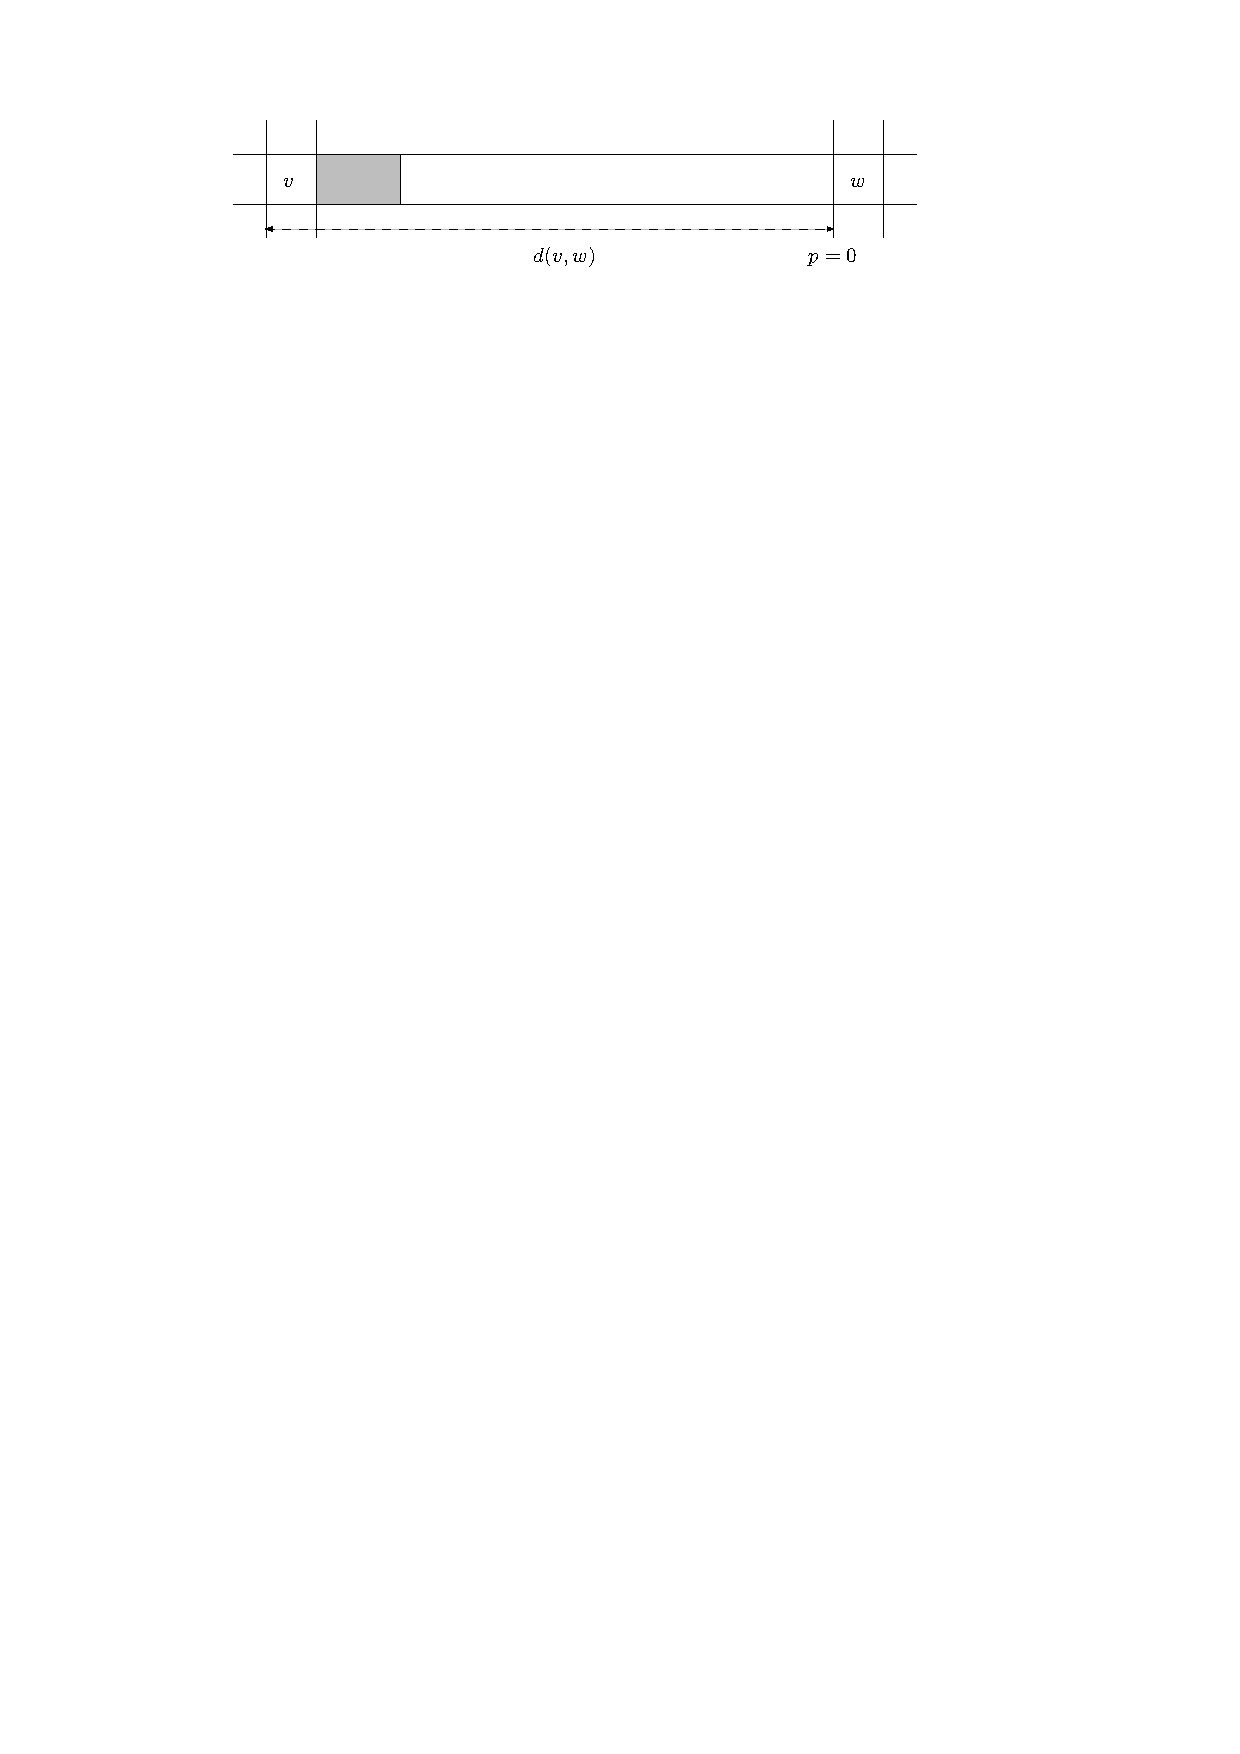
\includegraphics[width=1.0\textwidth]{figures/motion/tandem}
  }
  \caption{Tandem of two intersections $v$ and $w$ with lane of length $d(v,w)$.
    The grey rectangle represents some vehicle that just left intersection $v$.
    We assume that vehicles must drive at maximum speed as long as they occupy
    any intersection, so deceleration is only allowed from the shown position
    onwards.}
  \label{fig:tandem}
\end{figure}

When considering multiple vehicle driving between intersection, we can no longer
ignore the issue of road capacity, because the fact that only a limited number
of vehicles can drive or wait at the same time on a lane between intersections
may cause network-wide effects.
%
The capacity of lanes between intersections
is intimately related to the trajectories of vehicles, which we first want to
understand better. We have been using an optimal control formulation with the
objective that keeps the vehicles as close as possible to the next intersection
at all times (\texttt{MotionSynthesize}). This problem can be solved using
direct transcription, which works well enough if we just want to simulate the
behavior of the system. However, we believe that it is possible to explicitly
formulate the optimal controller. We will explain how to compute trajectories
corresponding to those obtained by direct transcription, but without using time
discretization.

Before we turn to the general case of networks of intersection, we will first
investigate the trajectories of vehicles in a tandem of two intersections as
depicted in Figure~\ref{fig:tandem}. Let $v$ denote the left intersection and
$w$ the right intersection and assume that vehicles drive from left to right.
% We will sometimes refer to intersection $w$ as the downstream intersection.
Furthermore, we will call the road segment strictly between both intersection
areas the \textit{lane}. To facilitate the following discussion, we will use $p$
to denote the position of a vehicle to distinguish it from the state
$x = (p, v)$, which also includes the velocity, and we fix position $p=0$ at the
stop-line of intersection $w$. Let the length and width of a vehicle $i$ be
denoted by $L_{i}$ and $W_{i}$, respectively. We measure the position of a
vehicle at the front bumper.
%
We will make the following assumption, that allow us to easily derive explicit
expressions of these trajectories.

\begin{assump}
  \label{assump:same_geometry}
  All vehicles have the same length $L_{i} = L$ and width $W_{i} = W$. Lanes
  are exactly $W$ units wide and are axis-aligned, such that intersection are
  squares.
\end{assump}

\begin{assump}
  \label{assump:full_speed}
  Vehicles must drive at full speed when entering an intersection and keep
  driving at full speed as long as they occupy an intersection.
\end{assump}

Now assume that some vehicle is scheduled to exit $v$ at time $t_{0}$ and to
enter $w$ at some time $t_{f}$. Let $p_{0} = -d(v,w) + W$ denote the position of
the vehicle when it starts to exit $v$. Let $y(t)$ denote the position of the
vehicle that drives in front of the current one, assuming there is one. To avoid
collision with this vehicle, the current vehicle must keep an appropriate
headway distance of at least $L$, so we enforce the \textit{safe headway}
constraint $p(t) + L \leq y(t)$ at all times.
%
In order to keep the vehicle as close to $w$ as possible at every time, while
respecting the double integrator vehicle dynamics
$\dot{p} = v, \, \ddot{p} = u$, we can generate a trajectory by solving the
optimal control problem
\begin{equation}
  \label{eq:optimal_control}
  \begin{aligned}
  \max_{u}    \quad & \int_{t_{0}}^{t_{f}} p(t) dt \\
  \begin{alignedat}{2}\text{s.t.}\\ {}\end{alignedat} \quad &\begin{alignedat}{2}
                     0 \leq \; &v(t) \leq v_{\max} , \\
                     {-a_{\max}} \leq \; &u(t) \leq a_{\max} , \\
                    p(t) + L \leq \; & y(t) , \\
                    \end{alignedat} \\
                    &\begin{alignedat}[t]{2}
                    & p(t_{0}) = p_{0} , &&  p(t_{f}) = 0 , \\
                    & v(t_{0}) = v_{\max} , \;\; && v(t_{f}) = v_{\max} .
                    \end{alignedat}
  \end{aligned}
\end{equation}
%
This problem can be solved by using direct transcription. After observing some
example solutions, we believe that the optimal controller is of the following
form.

\begin{proposition}
  \label{prop:optimal_control}
  Optimal control $u(t)$ for problem~\eqref{eq:optimal_control} switches between
  no acceleration and either full acceleration or full deceleration, i.e., we
  have a control function $u(t) := \ddot{x}(t)$ that satisfies
  $u(t) \in \{-a_{\max}, 0, a_{\max}\}$ and some sequence of alternating
  deceleration and acceleration periods, represented by some sequence of
  disjoint intervals
\begin{align*}
  (D_{0}, A_{1}, D_{1}, \dots, A_{n-1}, D_{n-1}, A_{n}) ,
\end{align*}
so that the optimal controller is given by
\begin{align}
  u(t) = \begin{cases}
           {-a_{\max}} &\text{ if } t \in D_{k} \text{ for some } k , \\
           \phantom{-} a_{\max}   &\text{ if } t \in A_{k} \text{ for some } k , \\
           \phantom{-} \;\, 0 &\text{ otherwise. }
         \end{cases}
\end{align}
\end{proposition}

We show that problem~\eqref{eq:optimal_control} is a special case of optimal
control problems of the form
\begin{align}
  \begin{split}
  \label{eq:state_constraints}
  \max \quad & \int_{t=0}^{T} F(x(t), u(t), t) dt \\
  \text{ s.t. } \;\, & \dot{x}(t) = f(x(t), u(t), t) , \quad x(0) = x_{0} , \\
                & g(x(t), u(t), t) \geq 0 , \\
             & h(x(t), t) \geq 0 , \\
             & a(x(T), T) \geq 0 , \\
             & b(x(T), T) = 0 ,
  \end{split}
\end{align}
where $x$ is the vector of state variables and $u$ is the control input.
%
Here, the constraints $g$ are called mixed state constraints, because they
involve both state and control variables, while constraints $h$ are called pure
state constraints.
%
Instead of writing $p$ and $v$ separately, we will now write the state as a
vector $x(t) = (x_{1}(t), x_{2}(t))$ with position $x_{1}(t)$ and velocity
$x_{2}(t)$. The control function $u(t)$ corresponds to acceleration. Without
loss of generality, we assume that $v_{\max} = 1$. The initial state is
$(p_{0}, 1)$ and the target state is $(0, 1)$.
%
Writing $y(t)$ for the state trajectory of the vehicle in front of the current
vehicle, optimal control problem~\eqref{eq:optimal_control} is equivalent
to~\eqref{eq:state_constraints} when setting\footnote{Instead of using quadratic
  expressions, both the mixed and the pure state constraint could have each been
  written as two linear constraints, e.g., we could have chosen
  $g(x, u, t) = (u_{\max} - u, u_{\max} + u)$. However, this does not satisfy
  the constraint qualification conditions of the theorem that we use in
  Section~\ref{sec:single_vehicle}}
\begin{align}
  \label{eq:settings}
\begin{split}
  F(x, u, t) &= x_{1} , \\
  f(x, u, t) &= (x_{2}, u) , \\
  x_{0} &= (p_{0}, 1) , \\
  g(x, u, t) &= u_{\max}^{2} - u^{2} , \\
  h_{1}(x, t) &= x_{2} - x_{2}^{2} , \\
  h_{2}(x, t) &= y_{1}(t) - x_{1} - L , \\
  b(x, t) &= (x_{1}, x_{2} - 1) .
\end{split}
\end{align}
%
% \begin{align*}
%   \max \int_{0}^{T} \underbrace{x_{1}(t)}_{F(x,u,t)} dt
% \end{align*}
% \begin{align*}
%   \dot{x} = f(x,u,t) = \begin{pmatrix} x_{2} \\ u \end{pmatrix} , \quad
%   x(0) = \begin{pmatrix}
%            p_{0} \\ 1
%          \end{pmatrix}
% \end{align*}
% \begin{align*}
%   -u_{\max} \leq u(t) \leq u_{\max} \quad &\iff \quad \underbrace{u_{\max}^{2} - u^{2}}_{g(x,u,t)} \geq 0 \\[1em]
%   0 \leq x_{2}(t) \leq 1 \quad &\iff \quad \underbrace{x_{2} - x_{2}^{2}}_{h(x,t)} \geq 0 \\[1em]
%   x(T) = \begin{pmatrix} 0 \\ 1 \end{pmatrix} \quad &\iff \quad
%   \underbrace{\begin{pmatrix}
%     x_{1}(T) \\ x_{2}(T) - 1
%   \end{pmatrix}}_{b(x(T), T)} = 0
% \end{align*}
%

\subsection{Special case: single vehicle}
\label{sec:single_vehicle}

Before we analyze problem~(\ref{eq:state_constraints}--\ref{eq:settings}) in the
general, we consider the situation in which the headway constraint $h_{2}$ can
be ignored, which might occur when the preceding vehicle is sufficiently far
away, or the current vehicle is the only vehicle in the system. In that case, we
can prove Proposition~\ref{prop:optimal_control} and provide explicit
expressions for $D_{k}$ and $A_{k}$ of the optimal trajectory.
%
% The proof uses a variant of the Pontryagin Maximum Principle, specifically
% tailored to problems with state
% constraints~\cite{hartlSurveyMaximumPrinciples1995}.
%
When dealing with optimal control problems, the Pontryagin Maximum Principle (PMP) provides a
family of first-order necessary conditions for optimality. We are going to apply
such a PMP-style necessary condition that deals with mixed and pure state
constraints to characterize the optimal control.
%
A common approach to deal with pure state inequality constraints $h$ is to
introduce a multiplier $\eta$ and append $\eta h$ to the Hamiltonian, which is
known as the direct adjoining approach. Instead, we use Theorem 5.1
from~\cite{hartlSurveyMaximumPrinciples1995} (see also (4.29)
in~\cite{sethiOptimalControlTheory2019}), which is a so-called indirect
adjoining approach, because the $\eta h^{1}$ is appended to the Hamiltonian,
where $h^{1}$ is defined as
\begin{align*}
  h^{1} = \frac{dh}{dt} = \frac{\partial h}{\partial x}f + \frac{\partial h}{\partial t} .
\end{align*}

\begin{proof}[Proof of Proposition~\ref{prop:optimal_control} without safe
  headway constraint]
The first derivate of pure state constraint $h_{1}$ is given by
\begin{align*}
  h_{1}^{1}(x, u, t) = u - 2x_{2} u ,
\end{align*}
which shows that $h_{1}$ is of first-order, because the control $u$ appears
after differentiating once.
%
By adjoining $\mu g + \eta h_{1}^{1}$ to the Hamiltonian
\begin{align*}
  H(x, u, \lambda, t) = F(x,u,t) + \lambda f(x,u,t) = x_{1} + \lambda_{1}x_{2} + \lambda_{2}u ,
\end{align*}
we obtain the Lagrangian in so-called Pontryagin form
\begin{align*}
  L(x, u, \lambda, \mu, \eta, t) &= H(x, u, \lambda, t) + \mu g(x, u, t) + \eta h_{1}^{1}(x, u, t) \\
  &= x_{1}  + \lambda_{1}x_{2} + \lambda_{2}u + \mu(u_{\max}^{2} - u^{2}) + \eta(u - 2x_{2}u) .
\end{align*}
%
Let $\{ x^{*}(t), u^{*}(t) \}$ denote an optimal pair for
problem~(\ref{eq:state_constraints}--\ref{eq:settings}), then this pair must
satisfy the necessary conditions in Theorem~5.1
from~\cite{hartlSurveyMaximumPrinciples1995}.
%
The Hamiltonian maximizing condition is
\begin{align*}
  H(x^{*}(t), u^{*}(t), \lambda(t), t) \geq H(x^{*}(t), u, \lambda(t), t)
\end{align*}
at each $t \in [0, T]$ for all $u$ with $g(x^{*}(t), u, t) \geq 0$ and satisfying
\begin{align*}
  h_{1}^{1}(x^{*}(t),u,t) \geq 0 \; \text{ whenever } \; h_{1}(x^{*}(t),u,t) = 0 .
\end{align*}
%
In our case, the latter condition reads
\begin{align*}
  u - 2x^{*}_{2}u \geq 0 \; \text{ whenever } \; x_{2}^{*} = \pm 1 ,
\end{align*}
%
which is satisfied by optimal controllers satisfying
\begin{align}
  \label{eq:optimal_u}
  \begin{split}
  u^{*}(t) =
  \begin{cases}
  u_{\max} &\text{ when } \lambda_{2}(t) > 0, \; x^{*}_{2}(t) < 1 , \\
  %0 \quad &\text{ when } \lambda_{2}(t) > 0, \; x^{*}_{2}(t) = 1 , \\
  -u_{\max} &\text{ when } \lambda_{2}(t) < 0, \; x^{*}_{2}(t) > - 1 , \\
  %0 &\text{ when } \lambda_{2}(t) < 0, \; x^{*}_{2}(t) = - 1 , \\
  0 &\text{ otherwise. }
  \end{cases}
  \end{split}
\end{align}

We now investigate what the costate trajectory should look like.
The adjoint equation is given by
\begin{align*}
  \dot{\lambda} = - L_{x}(x^{*}, u^{*}, \lambda, \mu, \eta, t) \iff
  \begin{cases}
    \dot{\lambda_{1}} = -1 , \\
    \dot{\lambda_{2}} = - \lambda_{1} + 2 \eta u^{*} .
  \end{cases}
\end{align*}
%
The Lagrange multipliers $\mu(t)$ and $\eta(t)$ must satisfy the complementary slackness conditions
\begin{align*}
  \mu (u_{\max}^{2} - {(u^{*})}^{2}) = 0 ,& \quad \mu \geq 0 , \\
  \eta (x_{2} - x_{2}^{2}) = 0 ,& \quad \eta \geq 0 \; \text{ and } \; \dot{\eta} \leq 0 .
\end{align*}
%
Whenever $u^{*} \neq 0$ on any open interval, then it is clear that we must have
$x_{2} \neq \pm 1$ on that interval, so the second complementary slackness
condition requires that we have $\eta = 0$. At isolated points where
$u^{*} \neq 0$, we can simply choose to set $\eta = 0$. Hence, $\eta u^{*} = 0$
everywhere and we have $\dot{\lambda_{2}}(t) = -\lambda_{1}(t) = t + c_{1}$ for
all $t \in [0, T]$, such that
$\lambda_{2}(t) = \frac{1}{2}t^{2} + c_{1}t + c_{2}$ for some constants
$c_{1}, c_{2}$.
%
In view of~\eqref{eq:optimal_u}, this shows that $u^{*}(t)$ has at most one
period of deceleration and at most one period of acceleration.
%
Assume $\lambda_{2}(t)$ has two zeros, which we denote by $t_{d}$ and $t_{a}$,
which give the start of the deceleration period and the start of the
acceleration period, respectively.

We now show how to compute $t_{a} - t_{d}$. Let $D$ denote the duration of the
deceleration, which must of course equal the length of the acceleration, because
$x_{2}(0) = x_{2}(T)$. Furthermore, $D$ must satisfy both $D \leq t_{a} - t_{d}$
and $D \leq 1 / u_{\max}$ and can thus be defined as the smallest of these two
bounds.
%
%We have $x_{1}^{*}(t) = t$ for $t \in [0, t_{d}]$.
From the vehicle dynamics follows that, for all $t \in [t_{d}, t_{d} + D]$ in
the deceleration period, we must have
\begin{align*}
  x_{2}^{*}(t) = 1 - u_{\max} (t-t_{d})
\end{align*}
and by integration, we obtain
\begin{align*}
  x_{1}^{*}(t) = x_{1}^{*}(t_{d}) + (t - t_{d}) - \frac{u_{\max}}{2}(t - t_{d})^{2} .
\end{align*}
%Next, $x_{1}^{*}(t) = x_{1}^{*}(t_{d} + D)$, for $t \in [t_{d} + D, t_{a}]$.
%
Similarly, for all $t \in [t_{a}, t_{a} + D]$ in the acceleration period, we must have
\begin{align*}
  x_{2}^{*}(t) = u_{\max} t
\end{align*}
and by integration, we obtain
\begin{align*}
  x_{1}^{*}(t) = x_{1}^{*}(t_{a}) + \frac{u_{\max}}{2}(t - t_{a})^{2} .
\end{align*}
%
Because the vehicle is stationary in $[t_{d} + D, t_{a}]$, we have
$x_{1}^{*}(t_{a}) = x_{1}^{*}(t_{d} + D)$.
It is now easily verified that we have
\begin{align*}
  x^{*}_{1}(T) = p_{0} + T + t_{d} - t_{a} .
\end{align*}
Recall that $x^{*}_{1}(T) = 0$, so we obtain $t_{a} - t_{d} = p_{0} + T$.

We now show that $t_{a}$ is uniquely determined.
%
From the complementary slackness conditions, we derive that
\begin{align*}
  \mu(t) = 0 \; & \text{ for } t \in (0, t_{d}) , \\
  \eta(t) = 0 \;& \text{ for } t \in (t_{d}, t_{d} + D) , \\
  \mu(t) = 0 \; & \text{ for } t \in (t_{d} + D, t_{a}) , \\
  \eta(t) = 0 \;& \text{ for } t \in (t_{a}, t_{a} + D) , \\
  \mu(t) = 0 \; & \text{ for } t \in (t_{a} + D, T) .
\end{align*}
%
Now together with the condition
\begin{align*}
  \frac{\partial L}{\partial u} |_{u=u^{*}(t)} = 0 \iff \lambda_{2} - 2 \mu u^{*} - 2 \eta x_{2} + \eta = 0 ,
\end{align*}
this shows that we can choose $\mu$ and $\eta$ such that $\mu(t) \geq 0$ and $\eta(t) \geq 0$ and
\begin{align*}
  \lambda_{2}(t) = \eta(t) \; & \text{ for } t \in (0, t_{d}) , \\
  \lambda_{2}(t) = -2 \mu(t) \; & \text{ for } t \in (t_{d}, t_{d} + D) , \\
  \lambda_{2}(t) = -\eta(t) \; & \text{ for } t \in (t_{d} + D, t_{a}) , \\
  \lambda_{2}(t) = 2 \mu(t) \; & \text{ for } t \in (t_{a}, t_{a} + D) , \\
  \lambda_{2}(t) = \eta(t) \;& \text{ for } t \in (t_{a} + D, T) .
\end{align*}
%
Suppose $t_{a} + D < T$, then for $t \in (t_{a} + D, T)$, we have
$\dot{\eta}(t) = \dot{\lambda_{2}}(t) > 0$, which contradicts the necessary
condition $\dot{\eta}(t) \leq 0$, hence $t_{a}= T - D$. This fixes a unique
costate trajectory $\lambda_{2}(t)$ and hence a unique optimal controller
$u^{*}(t)$ given by~\eqref{eq:optimal_u}.
\end{proof}


\begin{figure}
  \centering
  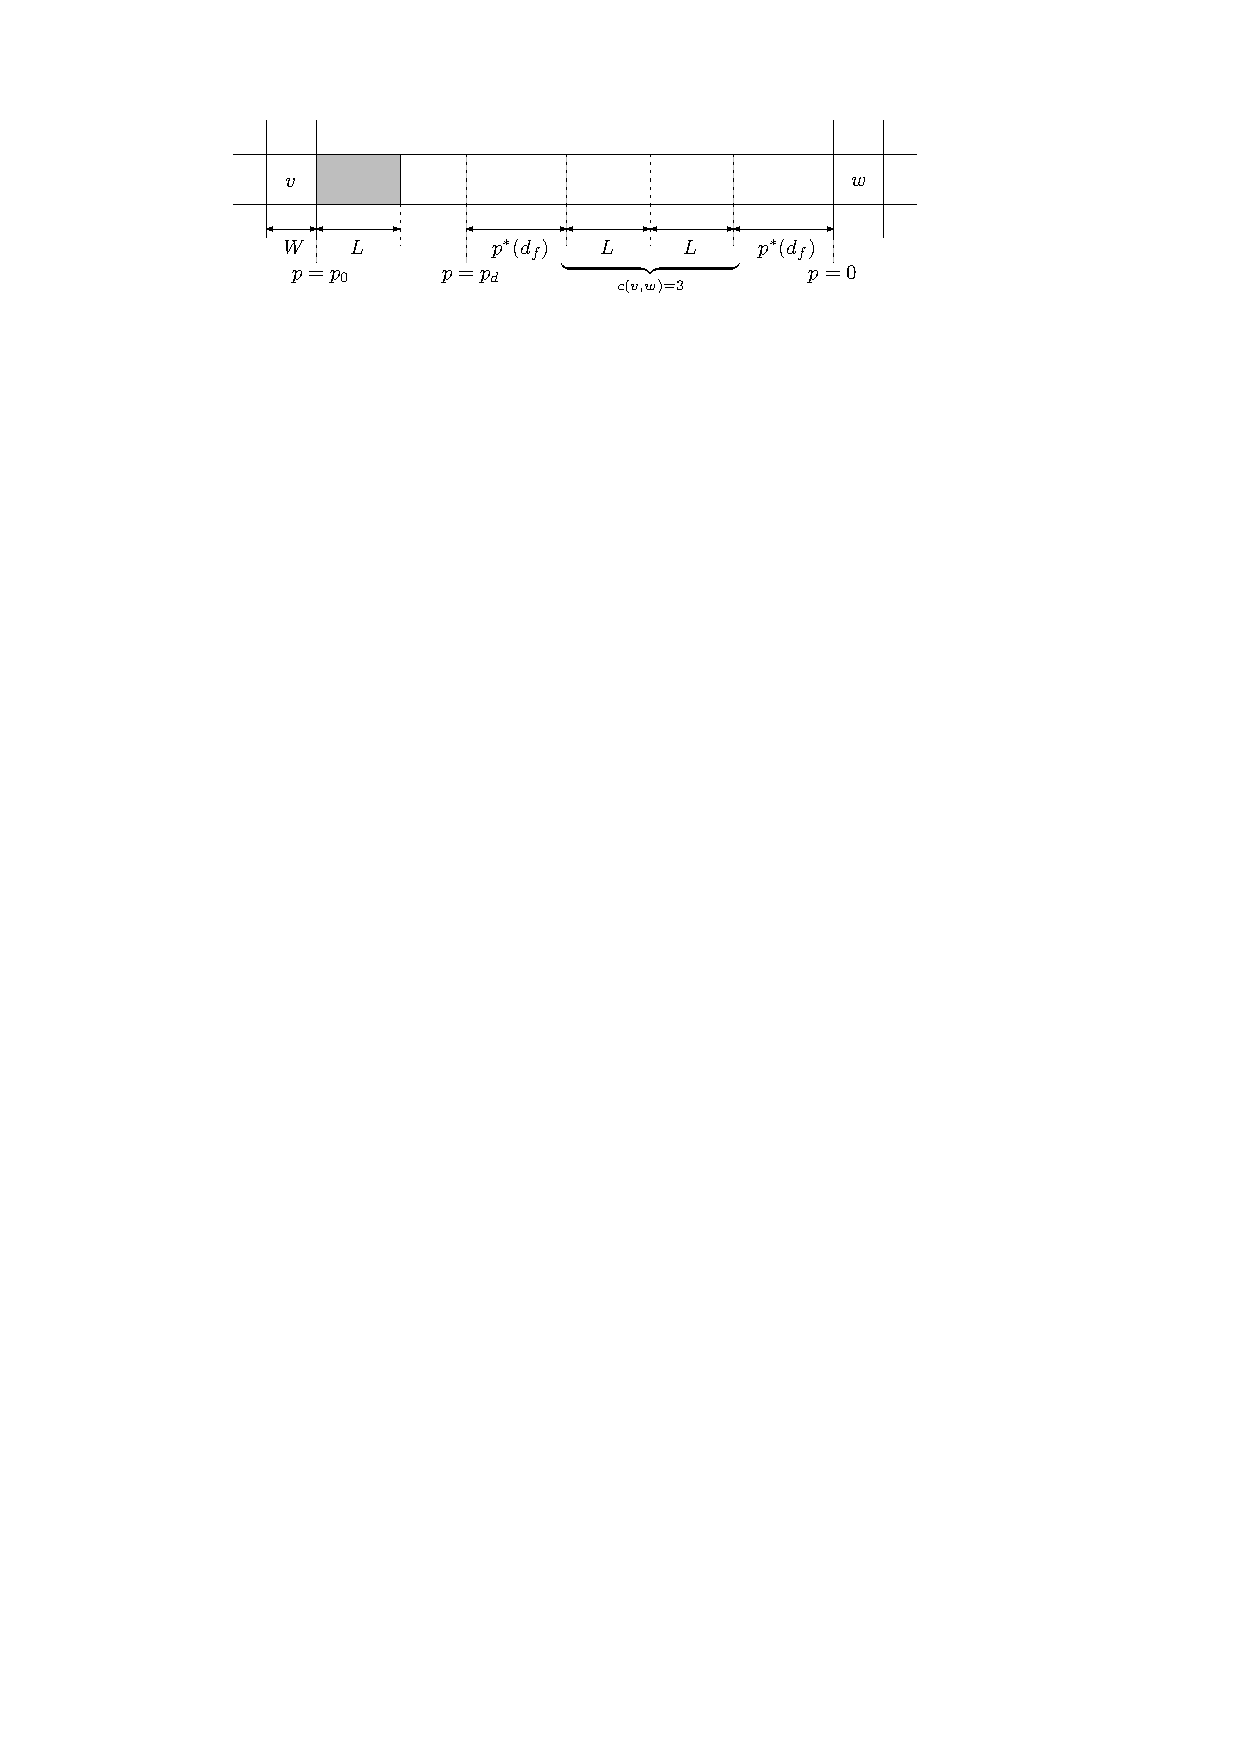
\includegraphics[width=0.99\textwidth]{figures/motion/tandem_annotated}
  \caption{Tandem of intersections with distances used in the determination of
    the lane capacity and the waiting positions.}
  \label{fig:tandem_annotated}
\end{figure}

\subsection{Multiple vehicles}

By observing optimal trajectories generated using direct transcription, we
observe that there is a lot of structure in how the trajectory of a vehicle
influences the trajectories of later vehicles. In this section, we provide a
direct way to explicitly calculate trajectories, without proving that these
trajectories are always feasible and optimal. Instead, we verify correctness of
our method numerically by comparing our explicit trajectories to the the output
of direct transcription for various system parameters and crossing times.

We start by investigating the limit on the number of vehicles that can occupy
the lane at the same time. Imagine that vehicles enter the lane until it is full
and then only after all vehicles have come to a full stop, they start to leave
the lane by crossing $w$.
%
Without any additional constraints, it follows from the vehicle dynamics that
the time it takes to fully accelerate from rest to maximum velocity is given by
$d_{f} = v_{\max} / a_{\max}$ and the corresponding full acceleration trajectory
is given by
\begin{align*}
  p^{*}(t) = a_{\max} t^{2} / 2 \quad \text{ for } 0 \leq t \leq d_{f} .
\end{align*}
To keep the presentation simple, we assume that maximum deceleration is also
$a_{\max}$, so it also takes $d_{f}$ time to fully decelerate from maximum
velocity to rest.
%
Suppose that we want to design the tandem network such that at least $c(v,w)$
vehicles can enter and decelerate to some waiting position, from which it is
also possible to accelerate again to full speed before crossing $w$.
%
Vehicles are required to drive at full speed as long as they occupy
any intersection. Therefore, a vehicle crossing $v$ can only start decelerating
after $p(t) \geq p_{0} + L$, so the earliest position where a vehicle can come to a
stop is $p = p_{0} + L + p^{*}(d_{f})$.
%
Because vehicles need to gain maximum speed before reaching $w$,
the position closest to $w$ where a vehicle can wait is $- p^{*}(d_{f})$.
%
Hence, in order to accomodate for $c(v,w)$ waiting vehicles, the length of the
lane must satisfy
\begin{align*}
  d(v, w) \geq W + L + 2p^{*}(d_{f}) + (c(v,w) - 1) L ,
\end{align*}
as illustrated in Figure~\ref{fig:tandem_annotated}.
%
Conversely, given the lane length $d(v,w)$, the corresponding lane capacity is
given by\footnote{Without Assumption~\ref{assump:same_geometry}, we cannot
  derive such a simple formula, because it would depend on the specific lengths
  of those vehicles currently in the system.}
\begin{align*}
  c(v, w) = \texttt{floor}\left( \frac{d(v,w) - W - 2 p^{*}(d_{f})}{L} \right) ,
\end{align*}
where $\texttt{floor}(x)$ denotes the largest integer smaller than or equal to
$x$.

% emphasize fixed locations
It turns out that the fixed locations where vehicles wait in the above scenario
are helpful in describing the optimal trajectories, even when vehicles never
fully stop. We will denote these fixed \textit{waiting positions} as
\begin{align*}
  p_{k} = - p^{*}(d_{f}) - (c(v,w) - k) L,
\end{align*}
for $k = 1, \dots, c(v,w)$.
%
Furthermore, let $p_{d} = p_{1} - p^{*}(d_{f})$ denote the position from
which vehicles must decelerate in order to stop at the earliest waiting position
$p_{1}$, which is the farthest from the destination intersection.
%
Now consider a vehicle that moves from $p_{k}$ to the next waiting position
$p_{k+1}$, so it moves exactly distance $L$. We consider such a start-stop
movement, without considering any safe following constraints. By symmetry of the
control constraints, the vehicle moves the same distance during both
acceleration and deceleration. Furthermore, the vehicle needs to be at rest at
the start and end of such trajectory. Hence, it is clear that it takes the same
amount of time $d_{s}$ to accelerate and decelerate. We assume that
$d_{s} < d_{f}$, which ensures that $v_{\max}$ is never reached during the
start-stop movement, which is illustrated in Figure~\ref{fig:start-stop}. In this case, it is
clear that we must have $L = 2 p^{*}(d_{s})$, from which we derive that
$d_{s} = \sqrt{L / a_{\max}}$.

\subsubsection{Ad-hoc approach}
We will now present a method to calculate the trajectory of a vehicle based on
its crossing times at $v$ and $w$ and the trajectory of the vehicle ahead of it.
We start from a sequence of deceleration and acceleration intervals that are
possibly overlapping and then merge them in pairs from left to right until they
become disjoint.
%
Specifically, let
\begin{align*}
  t_{d} := t_{0} + \frac{p_{d} - p_{0}}{v_{\max}}
\end{align*}
be the start of the initial deceleration interval
$D_{0} := [t_{d}, t_{d} + d_{f}]$, which is exactly the moment the vehicle needs
to start decelerating in order to stop at the first waiting position $p_{1}$, so
at time $t_{d}$ the vehicle is at position $p_{d}$. Similarly, let
$t_{a} = t_{f} - d_{f}$ be the start of the final acceleration interval
$A_{f} := [t_{a}, t_{f}]$. Now for every $k = 1, \dots, c(v,w) - 1$, we
consider a pair of start-stop intervals
$S_{k} := (A_{k}, D_{k}) = ([t_{k}, t_{k} + d_{s}], [t_{k} + d_{s}, t_{k} + 2 d_{s}])$
at some starting time $t_{k}$, moving the vehicle from $p_{k}$ to $p_{k+1}$. We
first show how to merge these intervals such that a sequence of disjoint
intervals is obtained. Afterwards, we show how times $t_{k}$ follow from the
trajectory of the vehicle ahead.

% show how to merge, assuming $S_{n}$ are disjoint
First, we show how to merge $D_{0}$ and $S_{1}$.
% case 1: separate
When we have $t_{d} + d_{f} \leq t_{1}$, it is clear that both parts are already
completely disjoint, so we do not have to do anything further.
% case 2: merging
When $t_{d}$ and $t_{1}$ are closer than $d_{f}$, we need to merge $D_{0}$
and $A_{1}$. In this case, we observe that $D_{0}$ gets shorter
at the end by some $\epsilon$ and the acceleration part of $S_{1}$ gets shorter at the
beginning, also by the same amount $\epsilon$, because the velocities must match. More
precisely, we construct two new consecutive intervals
\begin{align*}
  D_{0}' &= [t_{1} + 2 \epsilon - d_{f}, \; t_{1} + \epsilon] , \\
  A_{1}' &= [t_{1} + \epsilon,   \; t_{1} + d_{s}],  \\
  D_{1}  &= [t_{1} + d_{s},      \; t_{1} + 2 d_{s}] .
\end{align*}
%
We now determine $\epsilon$ as a function of $t_{1} - t_{d}$.
%
Because $D_{0}'$ and $A_{1}'$ are both $\epsilon$ shorter, the total distance
that is traversed is now $2 p^{*}(\epsilon)$ shorter. This means that the start
of $D_{0}'$ should be $2 p^{*}(\epsilon) / v_{\max}$ later than $t_{d}$, which
gives equation
\begin{align*}
  t_{d} + \frac{2 p^{*}(\epsilon)}{v_{\max}}  = t_{1} + 2\epsilon - d_{f} ,
\end{align*}
which is quadratic in $\epsilon$. Because we must have $\epsilon < d_{f}$, we need the
smallest solution
\begin{align*}
  \epsilon = d_{f} - \sqrt{d_{f} (t_{1} - t_{d})} .
\end{align*}
% case 3: merged
When we keep increasing $t_{d}$ while keeping $t_{1}$ fixed, we observe that
eventually part $A_{1}$ will completely disappear and $D_{0}$ and $D_{1}$ will
become a single interval, which is easily seen to happen when $\epsilon \geq d_{s}$.
Equivalently, this happens when $t_{d}$ is such that
$t_{d} \geq t_{1} - d_{f} + 2 d_{s} - 2p^{*}(d_{s}) / v_{\max}$.

% merge start-stops (AD-AD)
We now show how two start-stop parts have to be merged if they overlap. Consider
two start-stop parts $A_{k},D_{k}$ and $A_{k+1},D_{k+1}$ and suppose that
$t_{k} + 2 d_{s} < t_{k+1}$ such that both parts have to be merged. The parts
$D_{k}$ and $A_{k+1}$ merge by removing $\epsilon$ on both sides, similarly as
above. However, this causes the $D_{k},A_{k+1},D_{k+1}$ parts to shift up.
Therefore, $A_{k}$ and $D_{k}$ each need to be lengthened at the side where they
meet by some $\delta$ to match this.
%
Hence, it turns out we have to use the intervals
\begin{align*}
  A_{k}' &= [t_{k}, t_{k} + d_{s} + \delta] , \\
  D_{k}' &= [t_{k} + d_{s} + \delta, t_{k+1} + \epsilon] , \\
  A_{k+1}' &= [t_{k+1} + \epsilon, t_{k+1} + d_{s} ] , \\
  D_{k+1} &= [t_{k+1}, t_{k+1} + d_{s}] .
\end{align*}
%
We have that $\epsilon$ and $\delta$ need to satisfy
\begin{align*}
  \begin{cases}
  2\delta + 2\epsilon = t_{k+1} - t_{k} , \\
  2p^{*}(d_{s}+\delta) - 2p^{*}(d_{s} - \epsilon) = L .
  \end{cases}
\end{align*}
Solving this system of equations yields
\begin{align*}
  \delta &= \frac{L / a_{\max}}{t_{k+1} - t_{k}} - d_{s} + \frac{t_{k+1} - t_{k}}{4} , \\
  \epsilon &= (t_{k+1} - t_{k}) / 2 - \delta .
\end{align*}
%

Finally, we consider the merge with the final acceleration bang.

Note that the above types of merging are enough to process the whole sequence of
bangs, because when the first merge of $D_{0}$ and $A_{1},D_{1}$ results in a
single $D_{1}'$ and there is a next $A_{2},D_{2}$, we are again in the first
situation.

% show how $S_{n}$ follow from predecessor
We now show how $t_{k}$ follow from the trajectory of the preceding vehicle.

\begin{figure}
  \centering
  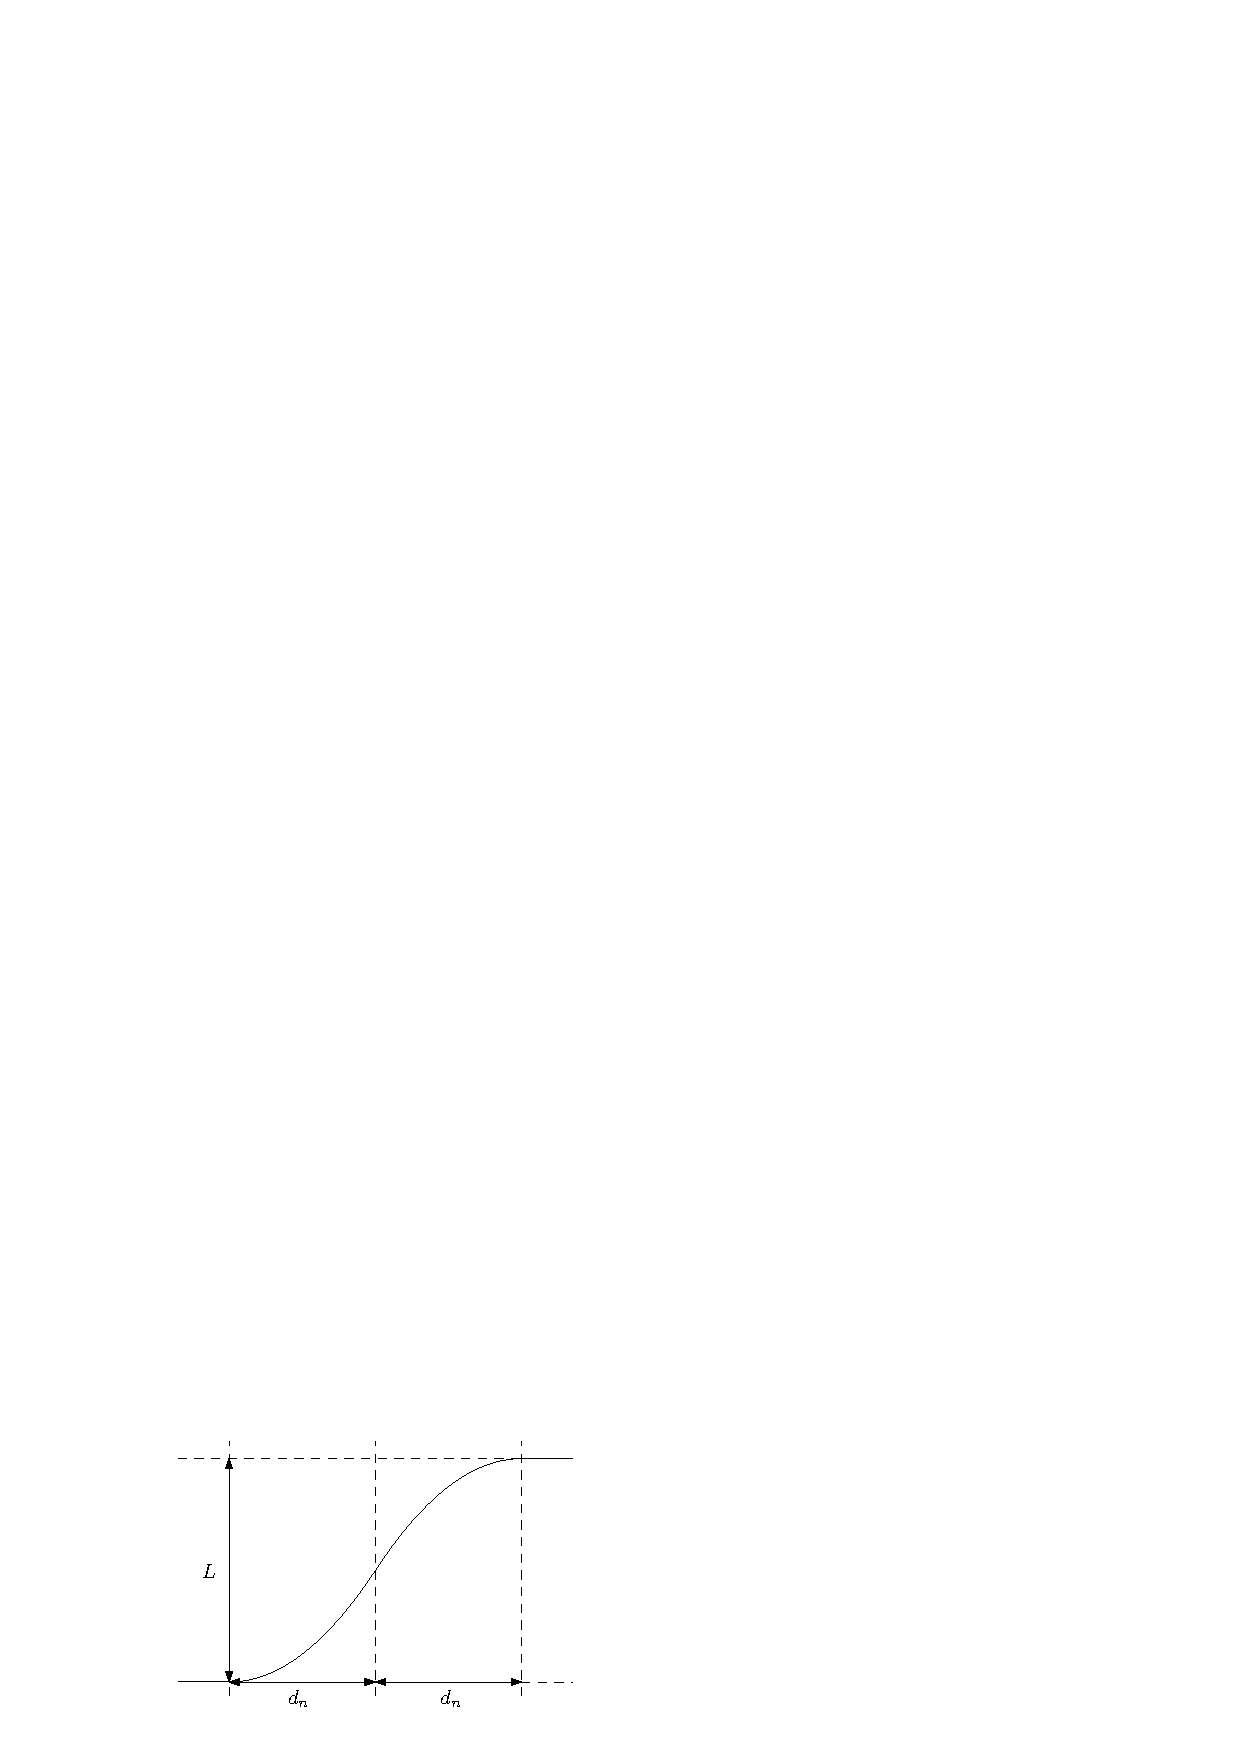
\includegraphics[scale=1.0]{figures/motion/start_stop_trajectory}
  \caption{Shape of some start-stop trajectory of a single isolate vehicle
    moving forward from some current waiting position $p_{k}$ to the next
    $p_{k+1}$.}
  \label{fig:start-stop}
\end{figure}

\begin{figure}
  \centering
  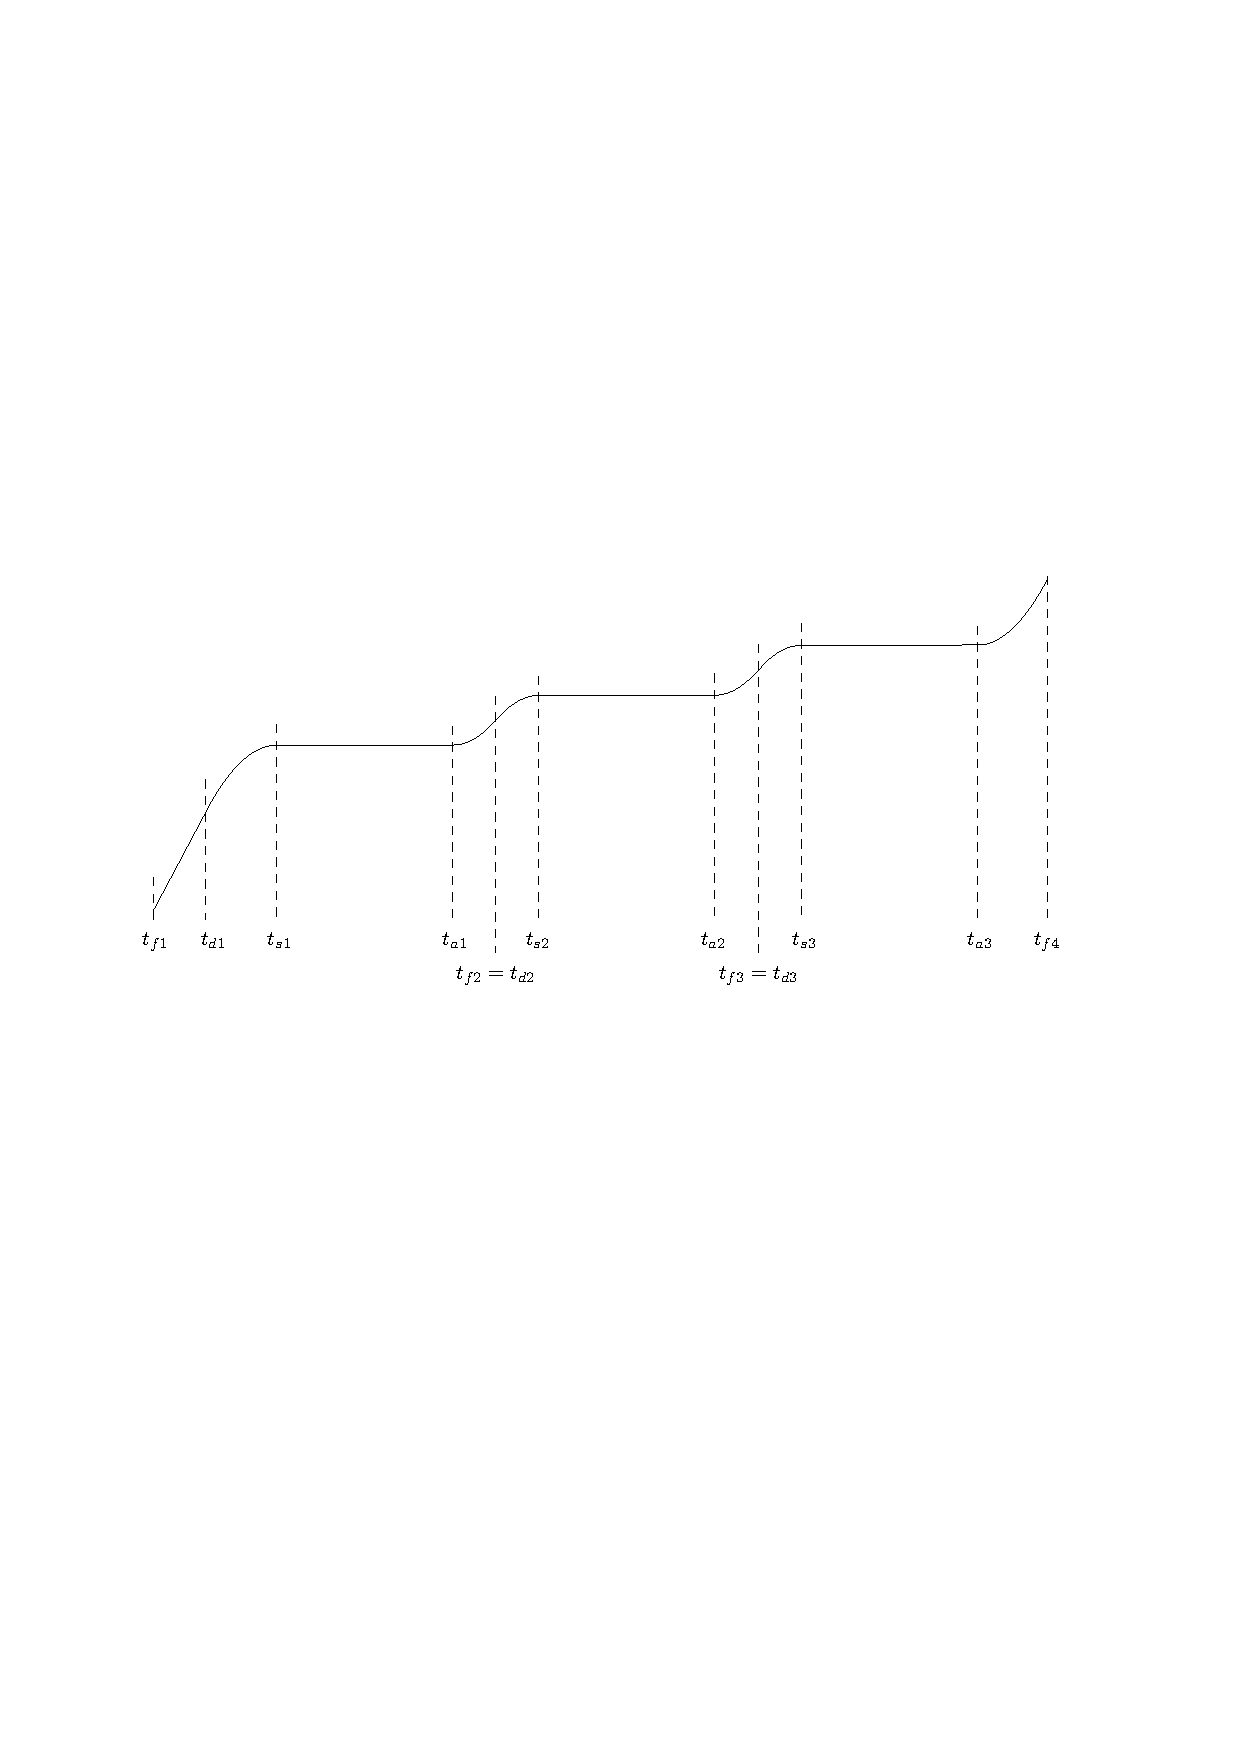
\includegraphics[width=0.8\textwidth]{figures/motion/tandem_trajectory}
  \caption{Sketch of vehicle trajectory in tandem with all the full start-stop
    parts unmerged.}
  \label{fig:tandem_trajectory}
\end{figure}

% \begin{figure}
%   \centering
%   \includegraphics[width=0.99\textwidth]{figures/motion/merge}
%   \caption{Sketch how the initial deceleration merges with the first start-stop phase.}
%   \label{fig:merge}
% \end{figure}

\newpage

\section{Trajectories in networks}

\begin{figure}
  \centering
  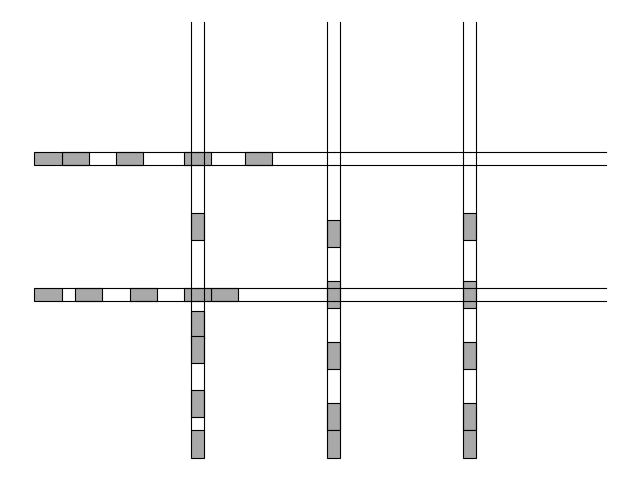
\includegraphics[width=0.55\textwidth]{figures/network/grid_example.png}
  \caption{Illustration of some grid-like network of intersections with vehicles
    drawn as grey rectangles. There are five vehicle routes: two from east to
    west and three from south to north. Turning at intersections is not
    allowed.}\label{fig:network_illustration}
\end{figure}

We now extend the single intersection model to a network of intersections
without turning routes, illustrated in Figure~\ref{fig:network_illustration}.
% network definition
We define a directed graph $(\bar{V},E)$ with nodes $\bar{V}$ and arcs $E$,
representing the possible paths that vehicles can follow. Nodes with only
outgoing arcs are \textit{entrypoints} and nodes with only incoming arcs are \textit{exitpoints}.
Let $V$ be the set of \textit{intersections}, which are all the nodes with
in-degree at least two.
%
Let $d(v, w)$ denote the distance between nodes $v$ and $w$.
%
For each route index $r \in \mathcal{R}$, we let
\begin{align*}
  \bar{V}_{r} = (v_{r}(0), v_{r}(1), \dots, v_{r}(m_{r}), v_{r}(m_{r+1}))
\end{align*}
be the path that vehicles $i \in \mathcal{N}_{r}$ follow through the network. We
require that the first node $v_{r}(0)$ is an entrypoint and that the last node
$v_{r}(m_{r+1})$ is an exitpoint and we write
\begin{align*}
  V_{r} = \bar{V}_{r} \setminus \{ v_{r}(0), \, v_{r}(m_{r+1}) \}
\end{align*}
to denote the path restricted to intersections. We say that some $(v, w) \in E$
is on path $V_{r}$ whenever $v$ and $w$ are two consecutive nodes on the path
and we write $E_{r}$ to denote the set of all these edges. We require that
routes can only overlap at nodes by making the following assumption.

\begin{assump}\label{assump:disjoint_routes}
  Every arc $(v,w) \in E$ is part of at most one route $V_{r}$.
\end{assump}

We start by considering networks in which all roads are axis-aligned such that
intersections always involve perpendicular lanes and where routes are such that
no turning is required. For each $v \in V_{r}$ define the conflict zone
$\mathcal{E}_{r}(v) = (b_{r}(v), e_{r}(v))$ and consider the union
\begin{align*}
  \mathcal{E}_{r} = \bigcup_{v \in V_{r}} \mathcal{E}_{r}(v)
\end{align*}
corresponding to the positions of vehicles $i \in \mathcal{N}_{r}$ for which it
occupies an intersection on its path $V_{r}$.
%
By reading $\mathcal{E}_{i} \equiv \mathcal{E}_{r}$ for $r(i) = r$, the single
intersection problem naturally extends to the network case. Like before, the
resulting problem can be numerically solved by a direct transcription method.

\subsection{General decomposition}
The general two-stage decomposition for the single intersection extends rather
naturally to the present model. Let for each pair $(i,v)$ of some vehicle
$i \in \mathcal{N}$ and an intersection $v \in V_{r(i)}$ along its route, let
\begin{align*}
\inf \{ t: x_{i}(t) \in \mathcal{E}_{r}(v) \} \;\; \text{ and } \; \sup \{ t: x_{i}(t) \in \mathcal{E}_{r}(v) \}
\end{align*}
be the crossing time and exit time, which we denote by $y(i,v)$ and
$y(i,v) + \sigma(i, v)$, respectively.
%
Instead of a single set of conflicts, we now define for each intersection
$v \in V$ in the network the set of conflict pairs
\begin{align*}
\mathcal{D}^{v} = \{ \{i,j\} \subset \mathcal{N} : r(i) \neq r(j), v \in V_{r(i)} \cap V_{r(j)} \} .
\end{align*}
Now the two-stage approach is to solve
\begin{align*}
  \min_{y,\sigma} \;\; & \sum_{r \in \mathcal{R}} F(y_{r}, \sigma_{r}) \\
  \text{ s.t. } & y(i,v) + \sigma(i,v) \leq y(j,v) \text{ or }  \\
                & y(j,v) + \sigma(j,v) \leq y(i,v) , & \text{ for all } \{i,j\} \in \mathcal{D}^{v} \text{ and } v \in V, \\
  & (y_{r}, \sigma_{r}) \in \mathcal{S}_{r} , \quad & \text{ for all } r \in \mathcal{R} ,
\end{align*}
%
where $F(y_{r}, \sigma_{r})$ and $\mathcal{S}_{r}$ are the value function and
set of feasible parameters, respectively, of the parametric trajectory
optimization problems
%
\begin{align*}
  F(y_{r}, \sigma_{r}) = \min_{x_{r}} & \; \sum_{r \in \mathcal{R}} J(x_{i}) \\
  \text{ s.t. } & x_{i}(t) \in D_{i}(s_{i,0}) , \quad & \text{ for } i \in \mathcal{N}_{r} , \\
  & x_{i}(y(i,v)) = b_{r}(v) , \quad & \text{ for } v \in V_{r} , i \in \mathcal{N}_{r} , \\
  & x_{i}(y(i,v) + \sigma(i,v)) = e_{r}(v) , \quad & \text{ for } v \in V_{r} , i \in \mathcal{N}_{r} , \\
  & x_{i}(t) - x_{j}(t) \geq L , \quad & \text{ for } (i, j) \in \mathcal{C} \cap \mathcal{N}_{r} ,
\end{align*}
where we again use subscript $r$ to group variables according to their associated route.


\subsection{Decomposition for delay objective}

Suppose we use use the crossing at the last intersection as performance measure, by defining the
objective function as
\begin{align*}
  J(x_{i}) = \inf \{ t: x_{i}(t) \in \mathcal{E}_{r}(v_{r}(m_{r}))\} .
\end{align*}
%
We show how to reduce the resulting problem to a scheduling problem, like we did
in the single intersection case.
%
We will again assume Assumption~\ref{assump:same_geometry} and
Assumption~\ref{assump:full_speed}, so vehicles will always cross intersections
at full speed, and all vehicles share the same geometry. Hence, the occupation
time $\sigma \equiv \sigma(i,v)$ is the same for all vehicles and intersections. For this
reason, we will write the shorthand $y_{r} \in \mathcal{S}_{r}$, because $\sigma_{r}$
is no longer a free variable.

As a consequence of Assumption~\ref{assump:same_geometry} and Assumption~\ref{assump:full_speed},
each lower-level trajectory optimization problem for a given route
$r \in \mathcal{R}$ decomposes into a sequence of problems, each corresponding to
two consecutive intersection along $V_{r}$.
%
This means that $y_{r} \in \mathcal{S}_{r}$ is equivalent to
$y_{(v,w)} \in \mathcal{S}_{(v,w)}$ for each $(v,w) \in E_{r}$, where
$y_{(v,w)}$ denotes the vector of all variables $y(i, v)$ and $y(i, w)$ for all
$i \in \mathcal{N}_{r}$ and $\mathcal{S}_{(v,w)}$ denotes the set of values of $y_{(v,w)}$ for which a feasible trajectory part can be found.
%
Hence, we will now focus on a tandem of two intersections and investigate the
trajectories of vehicles in this with the goal of stating sufficient conditions
for $y_{(v,w)} \in \mathcal{S}_{(v,w)}$.

\subsection{Crossing time scheduling as extension of job-shop scheduling}

The Job-Shop Scheduling Problem (JSSP) is a widely studied problem in which a
set of $n$ jobs must be assigned to non-overlapping time slots on a set of $m$
machines. Each job $i$ has a set of $n_{i}$ operations
$O_{i1}, \dots, O_{in_{i}}$ that need to be executed in this order. Each
operation $O_{ij}$ requires $p_{ij}$ processing time on machine $M_{ij}$. Each
machine can process at most one operation and early preemption is not allowed.
The task of the scheduler is to determine a valid schedule of start times
$y_{ij}$ for each operation, while minimizing some objective function. Let
$C_{ij} = y_{ij} + p_{ij}$ denote the \textit{completion time} of operation
$O_{ij}$, then the \textit{makespan} objective is given by the latest completion
time $\max_{i,j} C_{ij}$. Another objective is the \textit{total completion
  time}, given by
\begin{align*}
  \sum_{i=1}^{n} \sum_{j=1}^{m} C_{ij} ,
\end{align*}
which may be intuitively be thought of as representing some sort of total cost
of inventory, assuming we need to physically store jobs somewhere.

A commonly used representation of JSSP instances is the \textit{disjunctive
  graph} $G = (\mathcal{O}, \mathcal{C}, \mathcal{D})$, with vertices
$\mathcal{O} = \{ O_{ik} : 1 \leq i \leq n, 1 \leq k \leq n_{i} \}$
corresponding all the operations. The set of \textit{conjunctive arcs}
$\mathcal{C}$ encodes all the precedence constraints
$O_{i,k} \rightarrow O_{i,k+1} $ among each job's operations. The set of
\textit{disjunctive edges} $\mathcal{D}$ consists of undirected edges between
each pair of operations from distinct jobs that need to be processed on the same
machine, effectively encoding all such \textit{conflicts}. Each valid schedule
induces an ordering of operations on machines that is encoded by fixing the
direction of each disjunctive edge such that we obtain a direct acyclic graph.

\begin{itemize}
  \renewcommand\labelitemi{--}
{\color{gray}
% job-shop disjunctive graph
\item Introduce general job-shop problem and disjunctive graph, see Figure~\ref{fig:disjunctive_graph}.
% define travel constraints
\item Introduce travel constraints and its disjunctive graph arcs.
% define buffer constraints
\item Introduce buffer constraints and its disjunctive graph arcs.

% branch-and-bound
\item Formulate MILP problem and investigate how the solving time scales with network
size in terms of number of intersections and number of vehicles in the network.
Do the single intersection cutting planes still hold? Are there any obvious
cutting planes?
}
\end{itemize}

Let $y(i,v)$ denote the crossing time of vehicle $i$ at intersection $v \in V$.
Let $\mathcal{C}$ be the conjunctive pairs and let $\mathcal{D}^{v}$ denote the
disjunctive pairs at intersection $v \in V$.
%
Writing $\texttt{conj(\dots)}$ and $\texttt{disj}(\dots)$ for the usual
conjunctive and disjunctive constraints, we propose to solve the optimization
problem
\begin{subequations}\label{eq:network_problem}
\begin{align}
  \min_{y} \quad & \sum_{i \in \mathcal{N}} \sum_{v \in \mathcal{R}(l(i))} y(i,v) & \\
  \text{s.t.} \quad & r_{i} \leq y(i, v_{0}(l(i))) & \text{ for } i \in \mathcal{N} , \\
  & \texttt{conj}(y(i,v), y(j,v)) & \text{ for } (i,j) \in \mathcal{C}, v \in V , \\
  & \texttt{disj}(y(i,v), y(j,v)) & \text{ for } \{i,j\} \in \mathcal{D}^{v}, v \in V , \\
  & y(i, v) + d(v, w) \leq y(i, w) & \text{ for } i \in \mathcal{N}(l), (l, v, w) \in E, \label{eq:travel_delay} \\
  & y(i, w) + \rho(v, w) \leq y(j, v) & \text{ for } (i,j,v,w) \in \mathcal{F} , \label{eq:buffer_constraints}
\end{align}
\end{subequations}
where $\mathcal{F}$ is defined as
\begin{align*}
  \mathcal{F} = \{ (i,j,v,w) : i,j \in \mathcal{N}(l), k(i) + c(v,w) = k(j),  (l,v,w) \in E\}
\end{align*}
and we have $\rho(v, w) = c(v, w) L - d(v, w)$. Each $(i,j,v,w) \in \mathcal{F}$
represents a pair of vehicles driving on the same lane $(v,w)$, for which the
first vehicle must have made enough space in the lane before vehicle $j$ can
enter.


Lower bounds $\beta(i, v)$ on the crossing times of vehicles, where
$i = (r, k) \in \mathcal{N}$ is some vehicle index and $v \in V_{r}$.

There are two natural choices for the objective to optimize in this scheduling
setting.
%
We minimize the time each vehicle is in the system, which is equivalent to
minimizing the crossing time at the last intersection of each vehicle's route, written as
\begin{align*}
  \text{obj}_{1}(y) = \min \sum_{i \in \mathcal{N}} y(i, v_{r}(m_{r})) .
\end{align*}
Alternatively, it also makes sense to minimize the crossing time at every
intersection along each vehicle's route, so we can also minimize
\begin{align*}
  \text{obj}_{2}(y) = \min \sum_{i \in \mathcal{N}} \sum_{v \in V_{r(i)}} y(i, v) .
\end{align*}


\begin{figure}
  \centering
  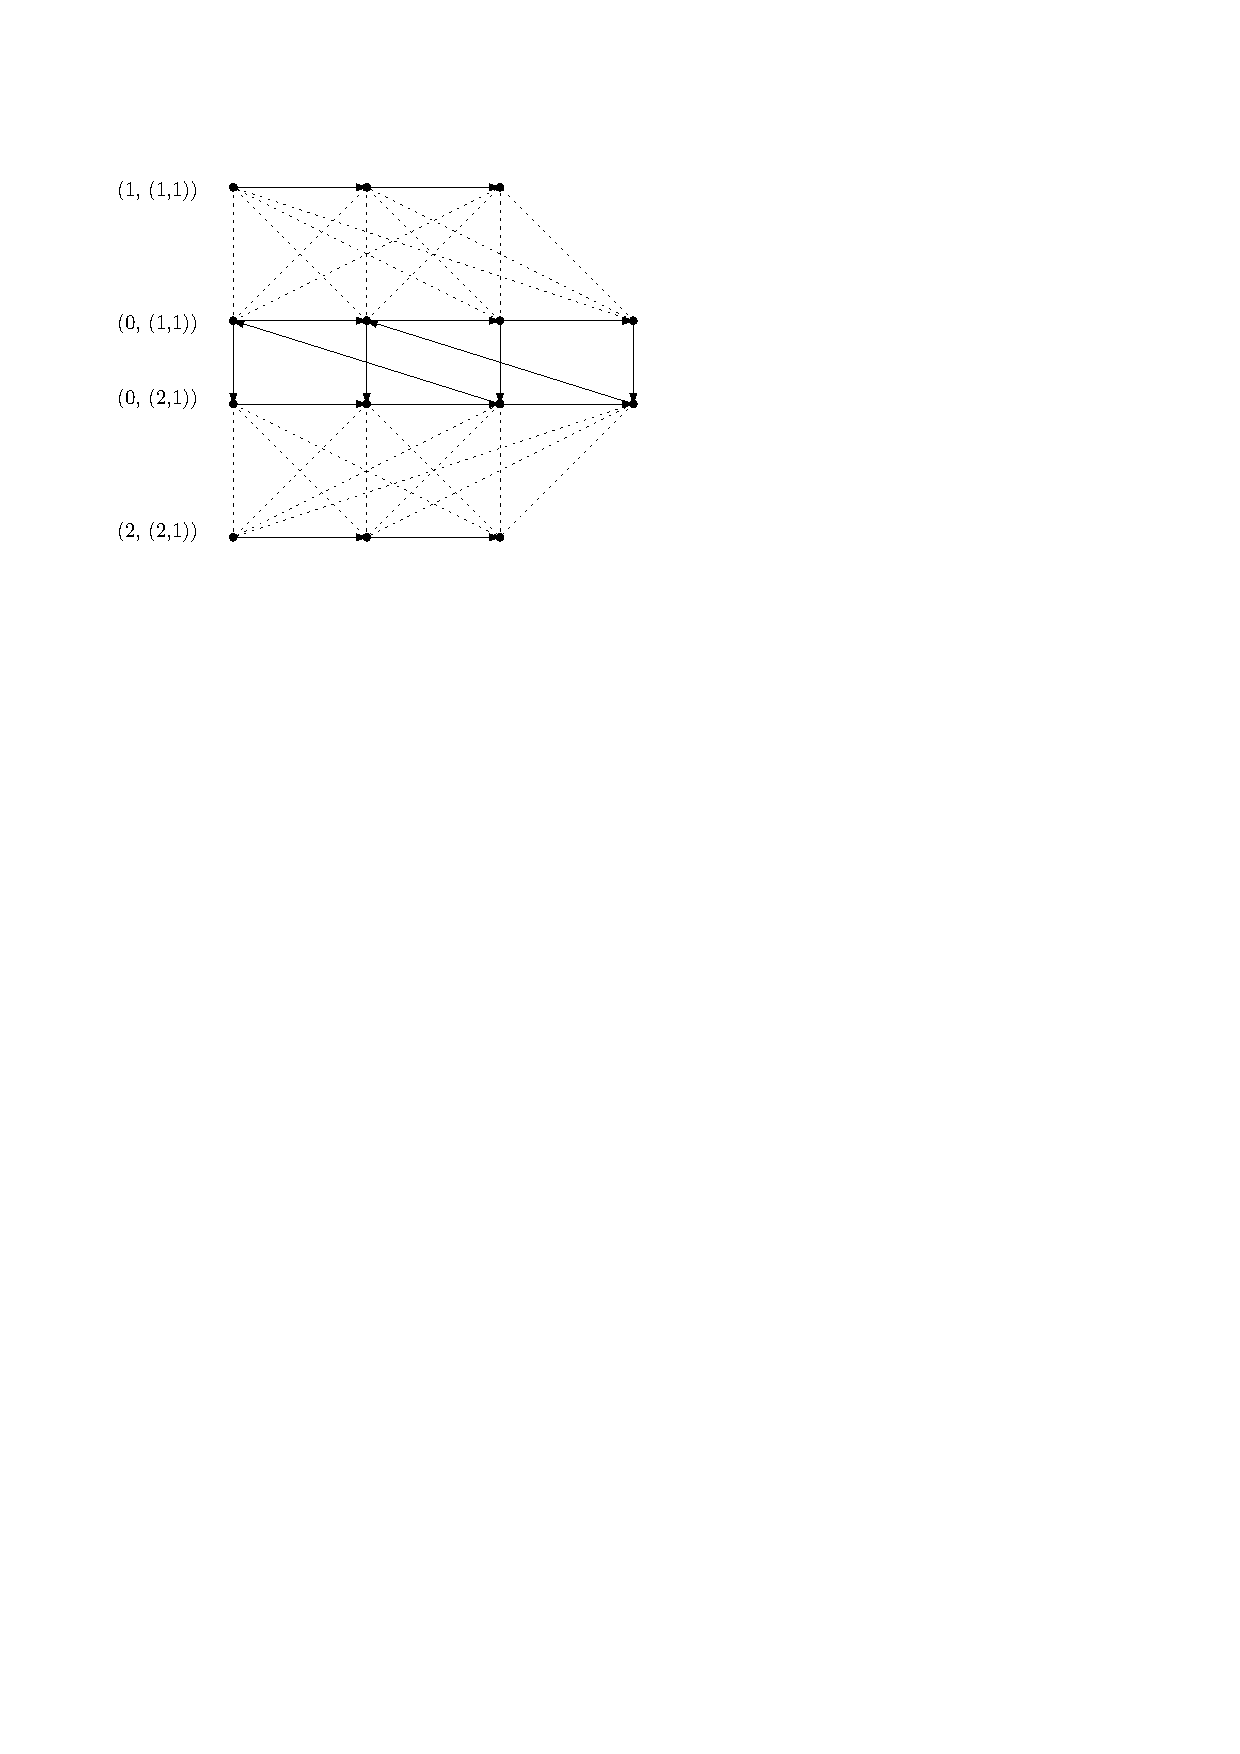
\includegraphics[scale=1]{figures/network/disjunctive_graph}
  \caption{Empty disjunctive graph belonging to a tandem of two intersections,
    labeled $v$ and $w$. There are three routes $\mathcal{R} = \{0, 1, 2\}$. On
    route 0, four vehicle are arriving, the other two routes have 3 arrivals
    each. Conjunctive arcs are drawn as from left to right, travel arcs are
    drawn from top to bottom and disjunctive arcs are drawn as dotted lines. Two
    buffer constraints are drawn as diagonal arcs, corresponding to a capacity
    of 2 vehicles for the lane between both intersections.}
  \label{fig:disjunctive_graph}
\end{figure}

\newpage
\section{Constructive heuristics}

Like in the single intersection case, we are going to model optimal solutions
using autoregressive models.
%
In the single intersection case, we argued that each schedule is uniquely
defined by its route order $\eta$. Generalizing this to the case of multiple
intersections, we see that a schedule is uniquely defined by the set of
route orders $\eta^{v}$ at each intersection $v \in V$. Instead of working with
such a set of sequences, we will intertwine the sequences to obtain a single
\textit{crossing sequence} $\eta$, which is a sequence of pairs $(r, v)$ of a
route $r \in \mathcal{R}$ at some intersection $v \in V_{r}$ and we will refer
to such a pair as a \textit{crossing}. Of course, this crossing sequence can be
constructed in many different ways, because it does not matter in which order
the intersections are considered, which is illustrated in Figure~\ref{fig:solution_equivalence}.
% \begin{align*}
%   | \{ t : \nu_{t} = v \} | = |\eta^{v}| \quad \text{ for each } v \in V ,
% \end{align*}
Given some problem instance $s$, we will consider autoregressive models of the form
\begin{align}
  \label{eq:autoregressive}
  p(\eta | s) =  \prod_{t=1}^{N} p(\eta_{t}| s, \eta_{1:t-1}) .
\end{align}

These models can also be understood in terms of a step-by-step schedule
construction process that transitions from a partial schedule state
$s_{t} = (s, \eta_{1:t})$ to the next state $s_{t+1}$ by selecting some
\textit{action} $\eta_{t} = (r_{t}, v_{t})$. We say a crossing is pending when
it still has unscheduled vehicles. Similarly, we say an intersection is pending
when some of its crossings are still pending. Therefore, the set of \textit{valid actions}
$\mathcal{A}(s_{t})$ at some intermediate state $s_{t}$ is exactly the set of
pending crossings.
%
% multiple correct actions
We again emphasize that multiple sequences of actions lead to the same schedule,
because the order in which intersections are considered does not matter for the
final schedule, which is illustrated in Figure~\ref{fig:solution_equivalence}.
%
The models that we study can be understood as being parameterized as some
function of the disjunctive graph $G_{t}$ of partial schedule $s_{t}$, so an
alternative way of writing~\eqref{eq:autoregressive} that emphasizes this is
\begin{align}
  p(\eta = ((r_{1}, v_{1}), \dots, (r_{N}, v_{N})) \; | \; s) = \prod_{t=1}^{N} p(r_{t}, v_{t} | G_{t-1}) .
\end{align}
%
Not all routes are valid at every intersection, so instead of modeling the joint
probability distribution $p(r_{t}, v_{t} | G_{t-1})$ over crossings, we apply
the chain rule to factorize this as
\begin{align}
  p(r_{t}, v_{t} | G_{t-1}) = p(r_{t} | v_{t} , G_{t-1}) p (v_{t} | G_{t-1}) .
\end{align}
In this case, the model $p(r_{t} | v_{t}, G_{t-1})$ can be thought of as
predicting a set of actions, one for each intersection.

\begin{figure}
  \centering
  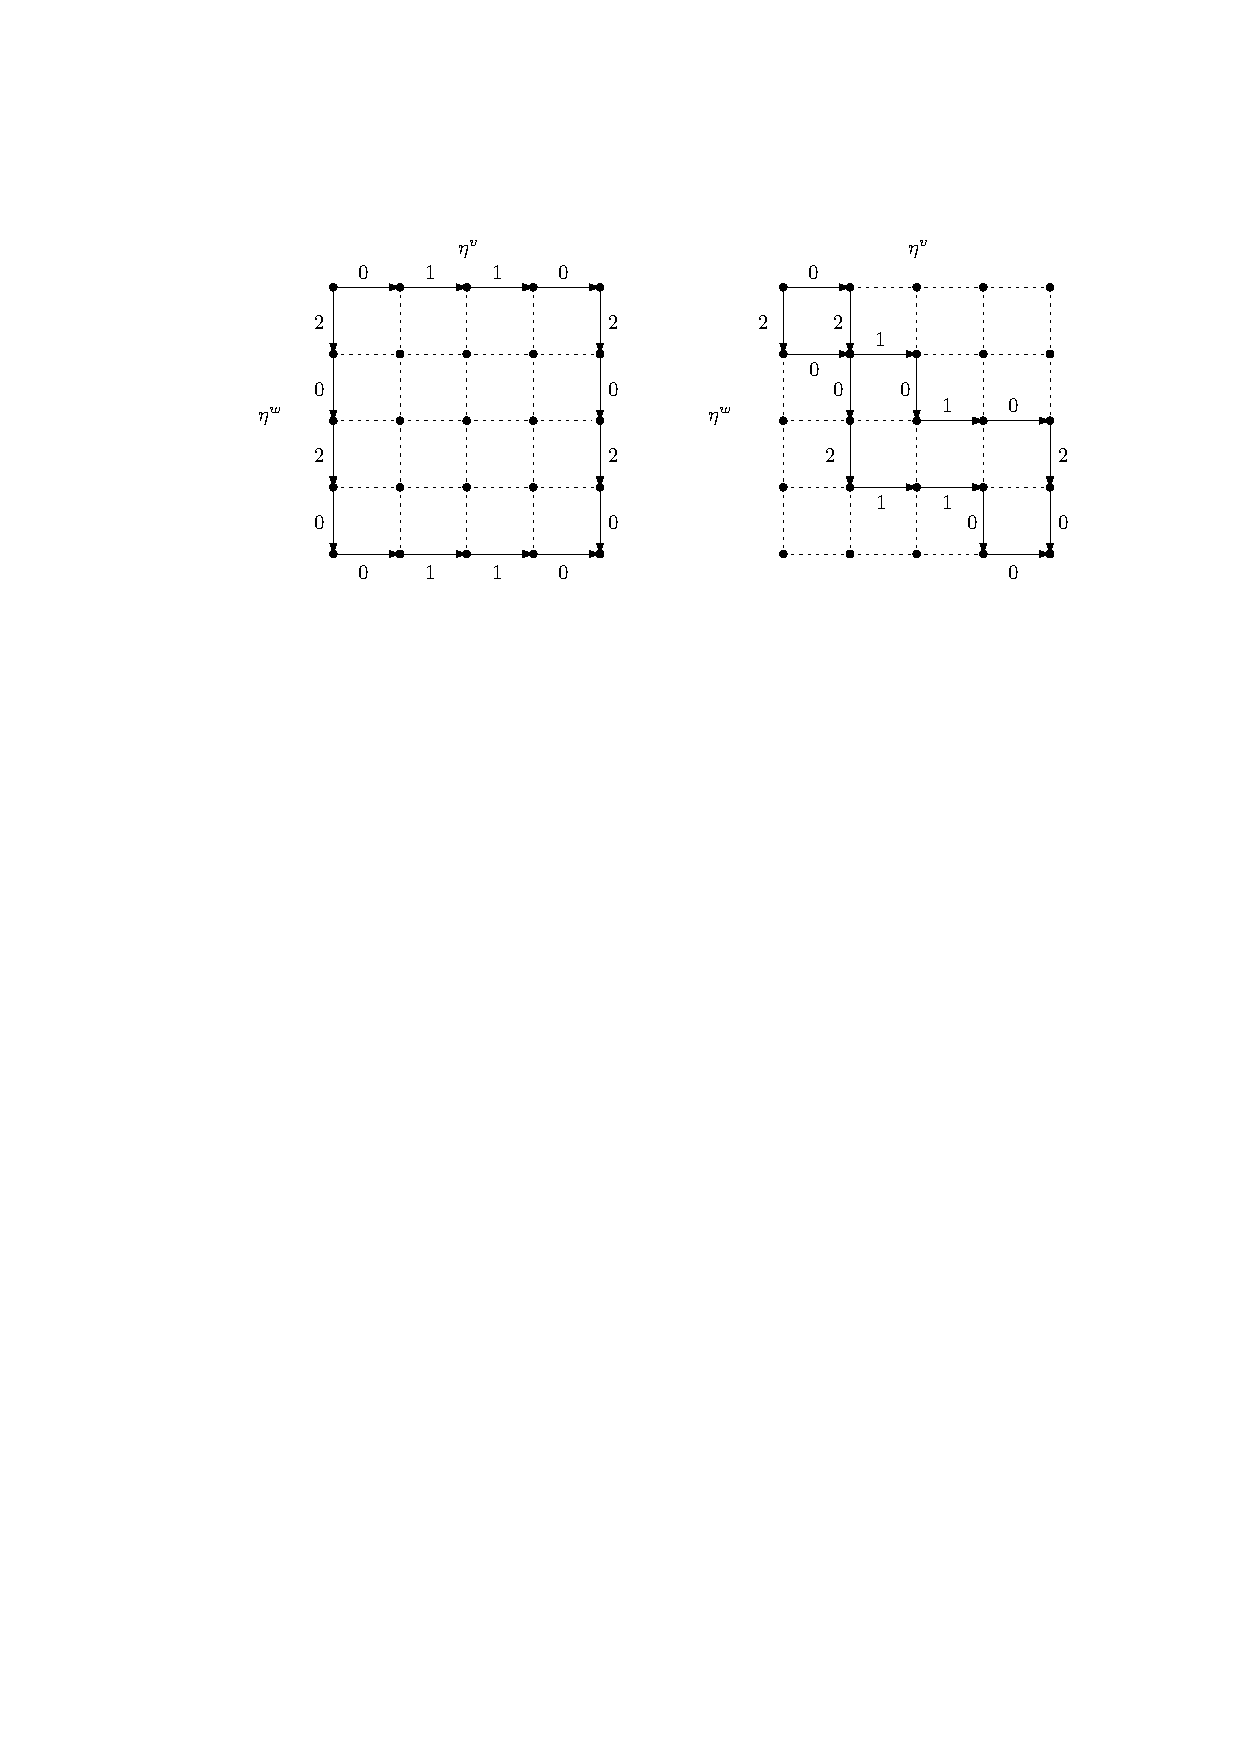
\includegraphics[width=0.9\textwidth]{figures/network/solution_equivalence}
  \caption{When each route order is locally fixed at every intersection, the
    global crossing sequence is not uniquely determined, because these local
    sequences may be merged in any order. Suppose we have a tandem of two
    intersections and a horizontal arrows correspond to taking the next local
    action at intersection $v$, a vertical arrows correspond to taking next
    local action at intersection $w$. Each valid crossing sequence corresponds
    to some path from the top-left to the bottom-right corner. Although any such
    crossing sequence produces the same schedule, it might be that our
    autoregressive model fits better on some sequences than others. For example,
    we might expect that sequences on the boundary of the grid, shown in the
    left grid, are harder to learn from data than sequences that stay closer to
    the diagonal, like in the right grid. The intuition is that we need to
    ``look into the future'' more to learn the former, while in the latter
    trajectories, progress in the two intersections is more balanced.}
  \label{fig:solution_equivalence}
\end{figure}

In the general class of autoregressive models for inputs and outputs with sets,
of which our model above is a special case (we have a set of sequences as
output), it has been noted before that the order in which inputs or outputs are
presented to the model during training has a considerable impact on the eventual
model fit~\cite{vinyalsOrderMattersSequence2016}.
%
For our model, we also expect to find such differences. Specifically, we will
investigate the impact of the order in which intersections are visited, which is
determined by $p(v_{t} | G_{t-1})$. We now propose some heuristic ways to define
$p(v_{t} | G_{t-1})$. Later, we will consider a neural network parameterization.
% random
First of all, the simple \textit{random} strategy would be to sample some
intersection with pending crossings at each step.
% ``boundary'' (or ``exhaustive'')
In the \textit{boundary} strategy, we keep visiting the same intersection until
it is done (when it has no pending crossings anymore), then move to some next
intersection. When the network of intersections is free of cycles, we could for
example follow some topological order. We use the term ``boundary'' because this
strategy produces trajectories along the boundary of the grid in
Figure~\ref{fig:solution_equivalence}.
% ``alternate''
In the \textit{alternating} strategy, we keep alternating between intersection to keep
the number of scheduled vehicles balanced among them. This produces trajectories
that can be understood as being close to the ``diagonal'' of the grid in
Figure~\ref{fig:solution_equivalence}. Again, the order in which we alternate between intersections may
again be based on some topological order.


\paragraph{Threshold heuristics.}
It is straightforward to extend the threshold rule to networks of
intersections, when assuming a fixed intersection order. Each time some
next intersection is visited, we apply the single intersection threshold rule to
pick the next route. This is straightforward to do, because we can just consider
the disjunctive subgraph induced by the nodes belonging to that intersection to
arrive at the single intersection case.
%
Furthermore, the definition of the threshold rule itself does not depend on the
network of intersections. This is a desirable property, because it allows us to
tune the threshold on small networks and then apply it on larger ones.


\subsection{Neural constructive heuristic}
\label{sec:neural_constructive}

We will now propose a neural network parameterization of
$p(r_{t} | v_{t}, G_{t-1})$ and train it based on optimal schedules in a
supervised learning setting. The model can be best understood as solving a
so-called multi-label classification problem, because it needs to provide a
distribution over routes at every intersection.
%
The training data set $\mathcal{X}$ consists of pairs
$(G_{t-1}, (r_{t}, v_{t}))$, to which we refer to as \textit{state-action} pairs
to draw the parallel with the terminology used in the reinforcement learning
literature.
%
To obtain these pairs, we sample a collection of problem instances, which are
solved to optimality using a MILP solver. For each optimal schedule, we compute
the corresponding optimal route order $\eta^{v}$ for each intersection.
%
From these, we can construct $\mathcal{X}$ in different ways.
% sample a single intersection order for each instance
For example, for each solved instance, we can randomly select some intersection
order $\mu$, which fixes the crossing order $\eta$. We can then replay
this sequence of actions step-by-step to obtain the corresponding sequence of
state-action pairs.
% multiple intersection order per instance
The model might become more robust when training on multiple samples of
intersections orders per instance.
% fixed intersection order
Alternatively, we can consider one of the fixed intersection orders
described at the start of this section (random, boundary, alternating).
% lookahead
Furthermore, combined with one of the above strategies, we can also employ some
kind of fixed lookahead procedure, as illustrated in
Figure~\ref{fig:state_action_collection}.
% inference
At inference time, we use the same intersection order as during training and at
each step we greedily select $r_{t}$.

\begin{figure}
  \centering
  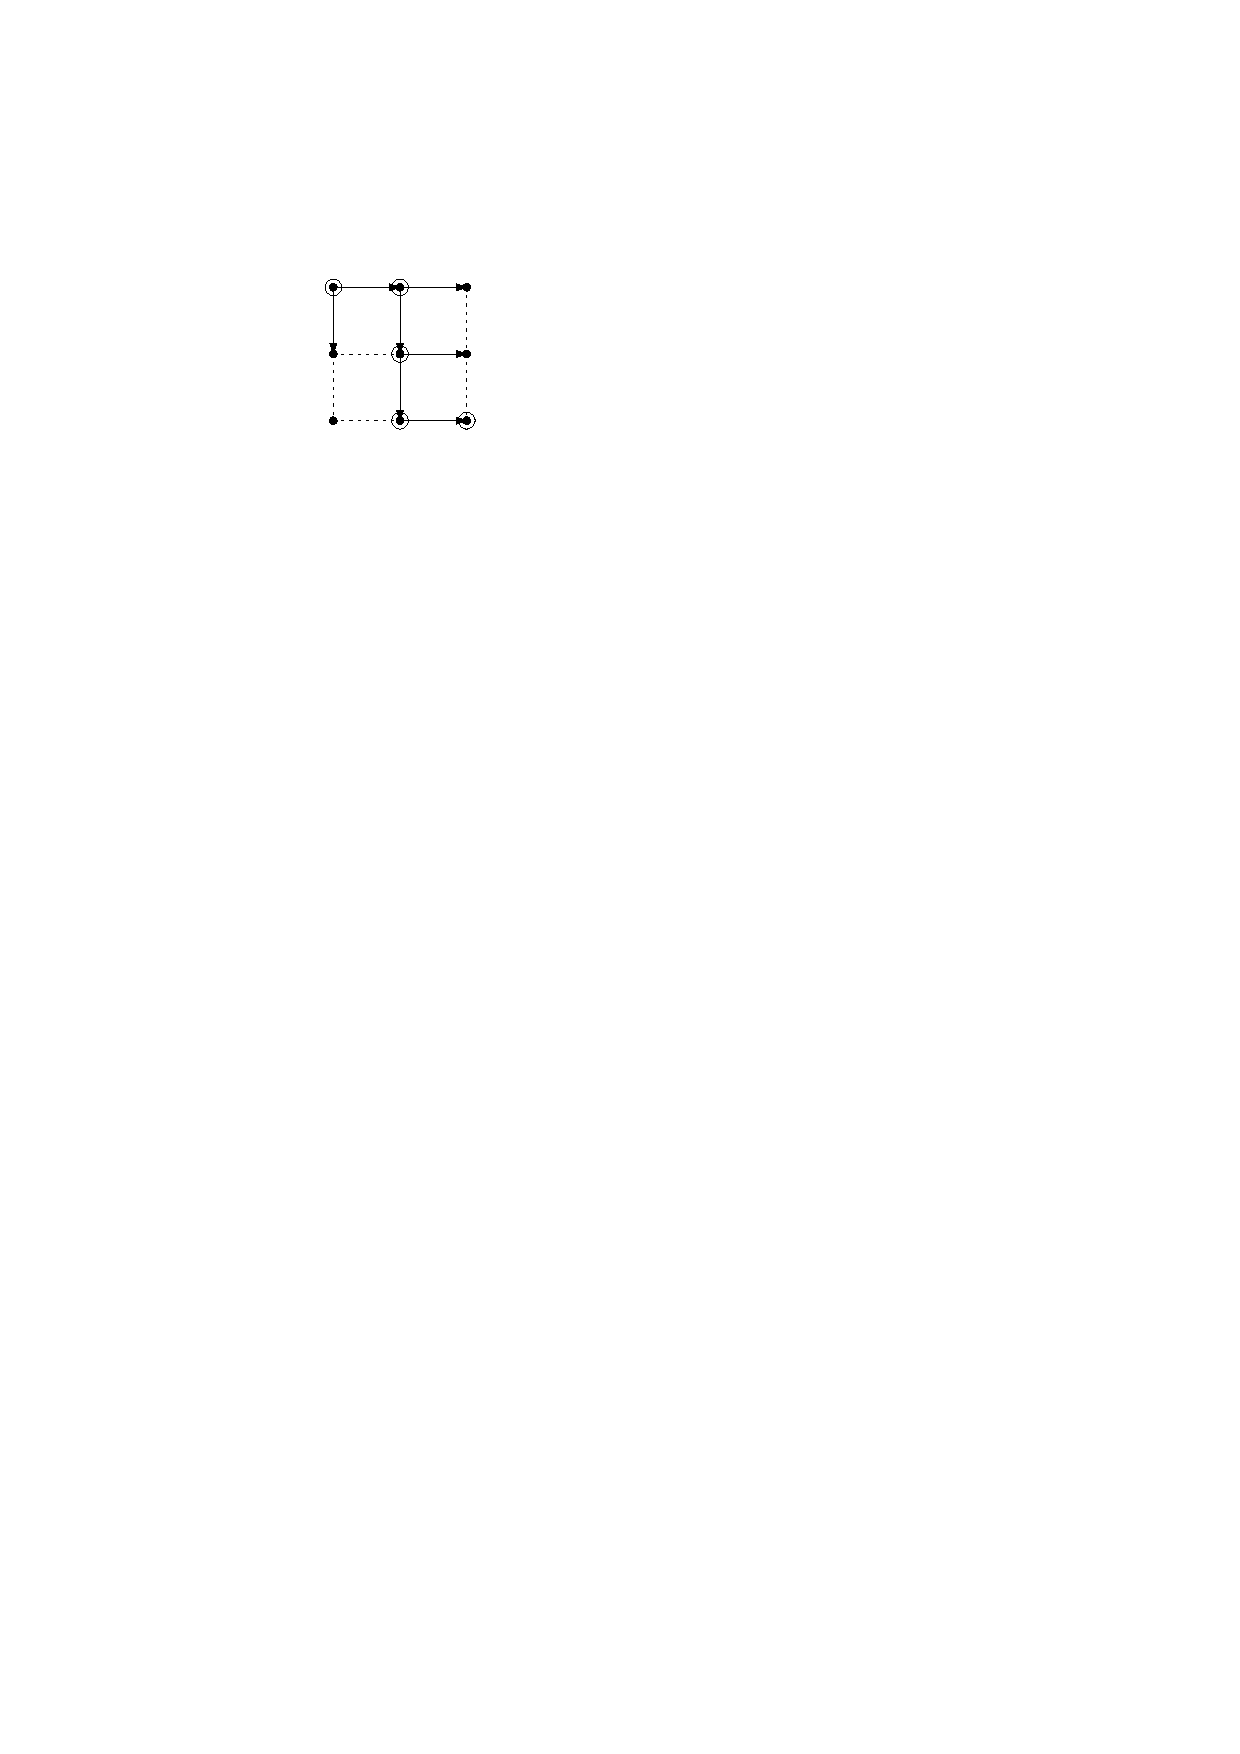
\includegraphics[scale=1.2]{figures/network/state_action_collection}
  \caption{Possible strategy for collecting state-action pairs: one action
    look-ahead. At every state $s_{t}$ with a set of possible actions
    $\mathcal{A}(s_{t})$, we add all state-action pairs
    $\{ (s, a) : a \in \mathcal{A}(s) \}$, but we pick a single action $a^{*}$
    to move to the next state. In the figure, the state-action pairs are
    depicted as solid arrows. The encircled dots are the states that are
    actually visited. Observe that this procedure can be naturally generalized
    to a look-ahead of arbitrary depth.}
  \label{fig:state_action_collection}
\end{figure}

We will now describe how the model is parameterized based on recurrent
embeddings of the sequences of crossing time lower bounds at each crossing, in a
somewhat similarly to how we used the horizons in the single intersection model.
%
Let $k(r, v)$ denote the number of scheduled vehicles at crossing $(r, v)$ and
let $n_{r}$ denote the total number of vehicles on route $r$. For each crossing
$(r, v)$, consider the earliest crossing time of the next unscheduled vehicle,
which we denote as
\begin{align*}
  T(r, v) = \beta(r, k(r, v) + 1, v) .
\end{align*}
We define the \textit{horizon} of crossing $(r, v)$ to be the sequence of relative lower bounds
\begin{align*}
  h(r, v) = (\beta(r, k(r, v) + 2, v) - T, \dots, \beta(r, n_{r}, v) - T) .
\end{align*}
%
Each such horizon is embedded using an Elman RNN. To produce a logit for each
crossing, these embeddings are fed through a feedforward network, consisting of
two hidden layers of size 128 and 64 neurons with relu activation and batch
normalization layers in between. See Figure~\ref{fig:rnn_model} for a schematic
overview of the architecture. {\color{Navy} Next: instead of $h(r, v)$, feed
  $(T(r, v), h(r, v))$ to the FF.}

\begin{figure}
  \centering
  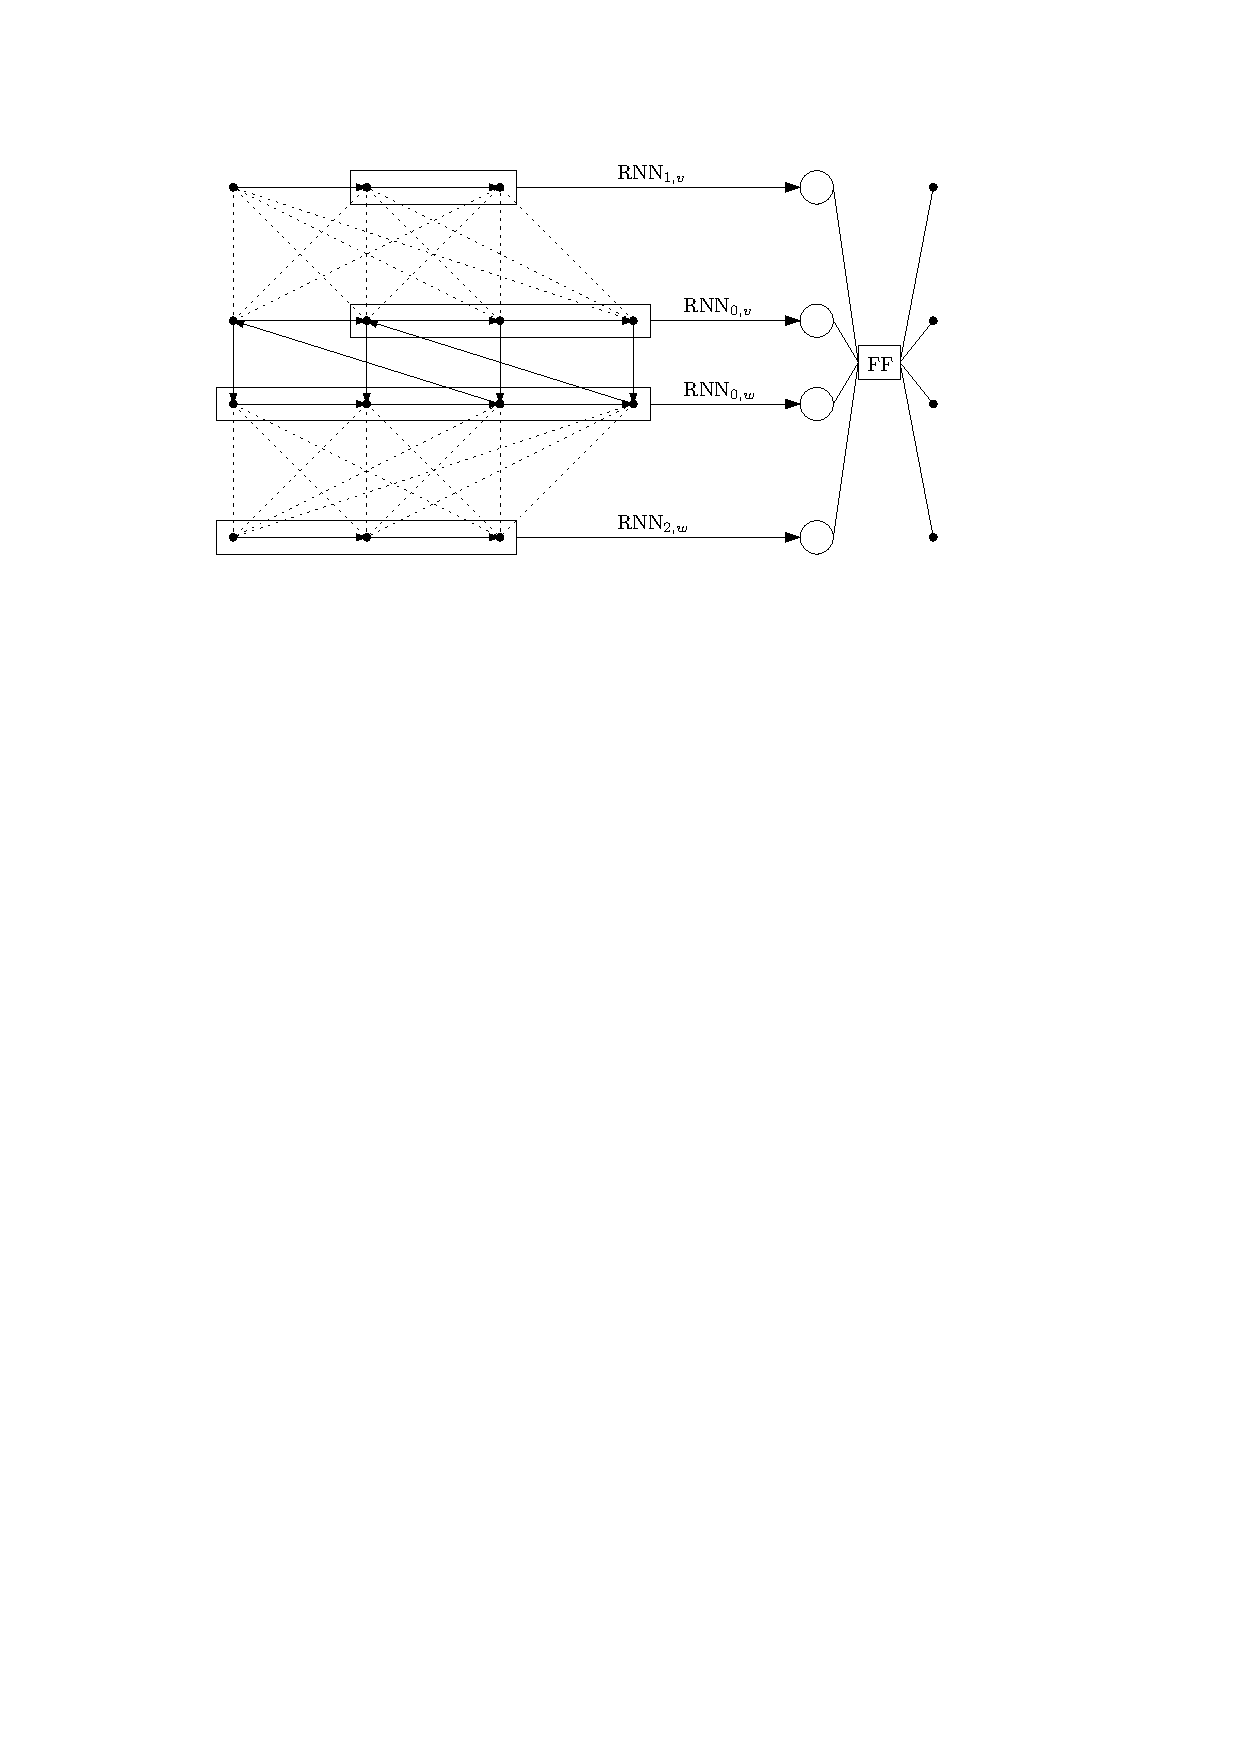
\includegraphics[scale=1]{figures/network/rnn_model}
  \caption{Illustration of model with RNN encoding of horizon at each crossing.
    The disjunctive graph nodes whose lower bounds are part of the current
    horizons are indicated with rectangles. The RNN embeddings (open circles)
    are fed through a final feedforward network to produce a logit (dots) for
    each crossing.}
  \label{fig:rnn_model}
\end{figure}

To train the model, we use the Adam optimizer with learning rate~$10^{-4}$ and a
batch size of $40$ state-action pairs. We experienced a case of the exploding
gradients problem when we did not use the batch normalization layers. To allow a fair comparison of methods accross instances of different
sizes, both in terms of the number of vehicles as the size of the network, we
adapt both objective as follows.
% objective variant 1
For the first variant, we define
\begin{align*}
  \text{obj}_{1}^{*}(y) = \frac{1}{|\mathcal{N}|}\min \sum_{i \in \mathcal{N}} y(i, v_{r}(m_{r})) - a(i, v_{r}(m_{r})) .
\end{align*}
Given some problem instance, let $N$ denote the length of a crossing sequence,
so it is also the total number of vehicle-intersection pairs $(i, v)$ that need
to be scheduled. For the second objective variant, we consider the average delay
per vehicle-intersection pair, as given by
\begin{align*}
  \text{obj}_{2}^{*}(y) = \frac{1}{N} \sum_{i \in \mathcal{N}} \sum_{v \in V_{r(i)}} y(i, v) - a(i, v) .
\end{align*}
For the current comparison we use $\text{obj}_{2}^{*}$, the results are listed
in Table~\ref{tab:results}.

% silent package loading


\begin{knitrout}
\definecolor{shadecolor}{rgb}{0.969, 0.969, 0.969}\color{fgcolor}\begin{table}
\centering
\caption{\label{tab:results}Average scaled optimal objective value computed using MILP and using the threshold heuristic with threshold $\tau = 0$. Each class of problem instances is identified by the number $n$ of vehicle arrivals per route and the grid network size as cols x rows.}
\centering
\resizebox{\ifdim\width>\linewidth\linewidth\else\width\fi}{!}{
\begin{tabular}[t]{cc|cc|c|c|c|ccc|cc|c|c|c|ccc|cc|c|c|c|ccc|cc|c|c|c|ccc|cc|c|c|c|ccc|cc|c|c|c|ccc|cc|c|c|c|ccc|cc|c|c|c|c}
\toprule
n & size & MILP & time & $\tau = 0$  (gap) & random (gap) & boundary (gap) & alternate (gap)\\
\midrule
5 & 2x1 & 57.27 & 0.06 & 65.27 (11.45\%) & 58.96 (2.95\%) & 58.72 (2.52\%) & 58.23 (1.66\%)\\
5 & 3x1 & 57.67 & 0.12 & 68.34 (15.44\%) & 59.77 (3.65\%) & 59.82 (3.74\%) & 58.72 (1.83\%)\\
5 & 3x2 & 57.35 & 1.38 & 69.17 (18.32\%) & 60.88 (6.16\%) & 60.36 (5.25\%) & 58.82 (2.56\%)\\
\bottomrule
\end{tabular}}
\end{table}

\end{knitrout}



\subsection{Reinforcement learning}

Instead of using a fixed training set $\mathcal{X}$ of state-action pairs during
training, we can fit our model from the perspective of a reinforcement learning
problem, which we already alluded to in Section~\ref{sec:neural_constructive}.
%
More precisely, given some scheduling problem instance $s$, we are dealing with
a Deterministic Markov Decision Process (DMDP), where partial disjunctive graphs
serve as states and actions correspond to crossings.
%
The potential benefit of using reinforcement learning is that we do not have to
fix an intersection order: our hope is that the training procedure will
automatically converge to some good intersection order.

{\color{Navy} The threshold heuristic ($\tau = 0$) can provide a
  \textit{baseline} for reinforcement learning, reducing the variance of the
  REINFORCE estimator.}

\newpage
\subsection{Network-agnostic architecture}

We now focus on models that generalize across network sizes. In particular, we
are interested in models that can be learned on relatively small networks (for
which exact solutions might be tractable) and can then be applied to larger
networks.

We use a GIN to compute an embedding for each node, which is then fed through an
MLP and softmax to produce a probability over nodes. The GNN computes node
embeddings, which are mapped to a score for each node. We compute the softmax
over the scores of the nodes and then compute the negative log likelihood loss
for backpropagation.
%
Like in Zhang et al., each action corresponds to a unique node, encoding the
operations that is dispatched next. However, we only really need to provide a
route-intersection pair, but how to exploit this in the policy model?
%
At this point, during the collection of observation-action pairs, we copy the
whole disjunctive graph for each state. Alternatively, we could use some sort of
masking for non-final states.



\bibliography{references}
\bibliographystyle{ieeetr}

\end{document}

% to enable the minted package
% Local Variables:
% TeX-command-extra-options: "-shell-escape"
% End:
